\chapter{Vanishing Nodes: correlation between hidden nodes}
\label{why}

In this section, the correlation of hidden-layer neurons is investigated.
If a pair of neurons is highly correlated (for example, the correlation coefficient is equal to $+1$ or $-1$), one of the neurons becomes redundant.
Great similarity between nodes may reduce the effective number of neurons within a network.
In some cases, the correlation of hidden nodes may disable the entire network. This phenomenon is called \textit{Vanishing Nodes}.

% In this section, we would like to show the importance of correlation of hidden layer nodes.
% We will define the correlation metric, show that the highly correlated hidden nodes may reduce the effective width of a neural network, and then connect the width of a network to its representation capability.
% We find that in some cases, the correlation of hidden nodes in a network may disable the whole network.
% We name this phenomena as \textit{vanishing nodes}, and we provide an intuitive example to demonstrate it.

First, consider a deep feed-forward neural network with depth $L$.
For simplicity of analysis, we assume all layers have the same width $N$.
The weight matrix of layer $l$ is $\mathbf{W}_l\in \mathbb{R}^{N\times N}$, the bias of layer $l$ is $\mathbf{b}_l\in \mathbb{R}^N$ (a column vector), and the common activation function of all layers is $\phi(\cdot):\mathbb{R}\rightarrow \mathbb{R}$. The input of the network is $\mathbf{x}_0$, and the nodes at output layer $L$ denote $\mathbf{x}_L$. The pre-activation of layer $l$ is $\mathbf{h}_l\in \mathbb{R}^N$ (a column vector), and the post-activation of layer $l$ is $\mathbf{x}_l\in \mathbb{R}^N$ (a column vector). That is, $\forall l \in \{1, ..., L\}$,

\begin{equation}
    \mathbf{h}_l=\mathbf{W}_l\mathbf{x}_{l-1}+\mathbf{b}_l,\;\;\;
    \mathbf{x}_{l}=\phi(\mathbf{h}_l).
\label{network_eqn}
\end{equation}

The variance of node $i$ is defined as $\sigma_i^2\overset{\Delta}{=}\mathbb{E}_{\mathbf{x}_0}[(x_{l(i)}-\overline{x_{l(i)}})^2]$, and the squared correlation coefficient ($\rho_{ij}^2$) between nodes $i$ and $j$ can be 
computed as 
\begin{equation}
\rho_{ij}^2\overset{\Delta}{=}
\frac
{\mathbb{E}_{\mathbf{x}_0}[(x_{l(i)}-\overline{x_{l(i)}})(x_{l(j)}-\overline{x_{l(j)}})]^2}
{\mathbb{E}_{\mathbf{x}_0}[(x_{l(i)}-\overline{x_{l(i)}})^2]\mathbb{E}_{\mathbf{x}_0}[(x_{l(j)}-\overline{x_{l(j)}})^2]},
\end{equation}
where $\rho_{ij}^2$ ranges from $0$ to $1$.
Nodes $x_{l(i)}$ and $x_{l(j)}$ are highly correlated only if the magnitude of the correlation coefficient between two nodes $\rho_{ij}$ is nearly 1. $\rho_{ij}^2$ indicates the magnitude of similarity between node $i$ and node $j$.
If $\rho_{ij}$ is close to $+1$ or $-1$, then node $i$ can be approximated in a linear fashion by node $j$.
Great similarity indicates redundancy.
If nodes of hidden layers exhibit great similarity, the effective number of nodes will be much lower than the original network width.
Therefore, we call this phenomena \textit{Vanishing Node Problem}.

Figure \ref{fig:sec4_sim11}, \ref{fig:sec4_sim1}, \ref{fig:sec4_sim12} and \ref{fig:sec4_sim13}
provide intuitives view of the vanishing node problem. The network
architecture is build with depth $L=100$, width $N\in\{6, 50, 100\}$ and activation functions
include $Linear$, $Hard$-$Tanh$ and $ReLU$.
The weight matrices are initialized with scaled-Gaussian and scaled-uniform initialization
(further discussion will provide in Section \ref{comp:init}) and the biases are set to zeros.
The network is fed with 1000 random generated
data points drawn from the zero-mean white Gaussian distribution. After the forward propagation, we choose
6 output nodes from the output layer to plot scatter plots with the first output node.
It is obvious that the neurons in four Subfigures (a) are so linearly correlated that the
actual number of effective number of the six nodes is 1, while the neurons in four Subfigures (c)
seem to be uncorrelated to each others.
It implies that if the network width $N$ is relatively small (compared to the network depth
$L$), the output nodes may become highly correlated, and hence results in the vanishing node
problem.

% \begin{figure}
    \begin{minipage}[c]{0.4\textwidth}
        \caption{We use the product of many Gaussian-initialized matrices as our \textit{"correlated-initialized"} weight matrix. To show the levels of correlation versus the number of matrices in the product, we plot the averaged cosine similarities of weight vectors. Notice that the number of nodes $N$ in hidden layers are all 6.}
        \label{fig:sec3_sim1}
    \end{minipage}\hfill
    \begin{minipage}[c]{0.5\textwidth}
        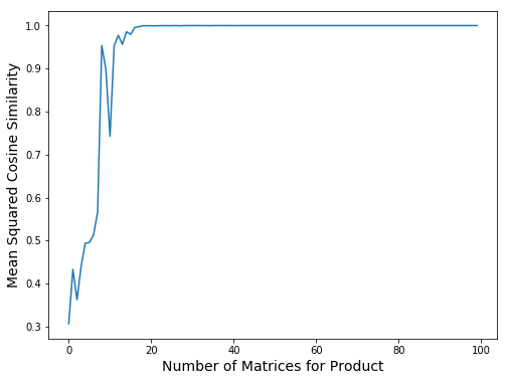
\includegraphics[width=\textwidth]{CorrelatedInitialization}
    \end{minipage}
\end{figure}

%\section{Results} \label{results}

In the following section, we propose a metric to measure the quantitative property of vanishing nodes for a deep feed-forward neural network.
Theoretical analysis of the metric indicates that the quantitative property of vanishing nodes is proportional to the network depth and inversely proportional to the network width.
The quantity is shown analytically to depend on the statistical property of weights and the nonlinear activation function. 

% In this section, we will (1) provide a theoretical analysis on the accumulation of the node correlation just after the weight initialization (2) give a numerical results for presenting that the weights update via back-propagation will intensify the node correlation.

%\section{Network Depth Makes Initial Correlations Accumulate} \label{initial}
\section{Vanishing Node Indicator} \label{initial}

Consider the network architecture defined in \eqref{network_eqn}. In addition, the following assumptions are
made: (1) The input $\mathbf{x}_0$ is zero-mean, and the features in $\mathbf{x}_0$ are independent and
identically distributed. (2) All weight matrices $\mathbf{W}_l$ in each layer are initialized from the same
distribution with variance $\sigma_w^2/N$. (3) All the bias vectors $\mathbf{b}_l$ in each layer are
initialized to zero.
% We would like to provide an analysis on the correlation of output nodes in a deep neural network. We will first setup a network, define a metric for measuring the correlation, perform theoretical analysis on the metric, and then provide several results of numerical simulations.

% To analyze the correlation of output layer nodes toward depth, we need to define a metric to measure the output layer node correlation.
% First, consider the network architecture we defined in \eqref{network_eqn}.
% In particular, we have made several assumptions: (1) The input $\mathbf{x}_0$ is zero-mean, and features in $\mathbf{x}_0$ are independent and identically distributed. (2) All the weight matrices $\mathbf{W}_l$ in each layer are initialized from a same distribution with variance $\sigma_w^2/N$. (3) All the bias vectors $\mathbf{b}_l$ in each layer are initialized to zero.

The input-output Jacobian matrix $\mathbf{J}\in\mathbb{R}^{N\times N}$  is defined as the first-order partial derivative of the output layer with respect to the input layer, which can be rewritten as
\begin{equation}
    \frac{\partial\mathbf{x}_L}{\partial\mathbf{x}_0}=\prod_{l=1}^{L}\mathbf{D}_l\mathbf{W}_l,
    \label{jacobian_eqn}
\end{equation}
where $\mathbf{D}_l\overset{\Delta}{=} diag(\phi'(\mathbf{h}_l))$ is the derivative of point-wise activation function $\phi$ at layer $l$.
% With the input-output Jacobian and the given assumptions, we can perform the first-order forward approximation:
To conduct a similar analysis as \cite{mft:linear}, consider the first-order forward approximation:
$\mathbf{x}_L-\overline{\mathbf{x}_L} \approx \mathbf{Jx}_0$. Therefore, the covariance matrix of the nodes ($\mathbf{C}\in\mathbb{R}^{N\times N}$) at the output layer  can be computed as

\begin{equation}
    \mathbf{C} \overset{\Delta}{=}
    \mathbb{E}_{\mathbf{x}_0}[(\mathbf{x}_L-\overline{\mathbf{x}_L})(\mathbf{x}_L-\overline{\mathbf{x}_L})^T]
    \approx
    \mathbb{E}_{\mathbf{x}_0}[(\mathbf{Jx}_0)(\mathbf{Jx}_0)^T]
    =
    \mathbf{J}\mathbb{E}_{\mathbf{x}_0}[\mathbf{x}_0\mathbf{x}_0^T]\mathbf{J}^T
    =
    \sigma_x^2\mathbf{J}\mathbf{J}^T,
    \label{covariance_eqn}
\end{equation}
where $\sigma_x^2$ is the common variance of features in $\mathbf{x}_0$, and the expected values are calculated with respect to the input $\mathbf{x}_0$. For notational simplicity, we omit the subscript $\mathbf{x}_0$ of the expectations in the following equations. 
It can be easily derived that the squared covariance of nodes $i$ and $j$ is equal to the product of the squared correlation coefficient and the two variances. That is, $[C_{(ij)}]^2=\rho_{ij}^2\sigma_i^2\sigma_j^2$.

In this paper, we propose the \textit{Vanishing Node Indicator (VNI)} $R_{sq}$ to quantitatively characterize the degree of vanishing nodes for a given network architecture. It is defined as follows:

\begin{equation}
    R_{sq}\overset{\Delta}{=}
    \frac{\sum_{i=1}^N\sum_{j=1}^N\rho_{ij}^2\sigma_i^2\sigma_j^2}
{\sum_{i=1}^N\sum_{j=1}^N\sigma_i^2\sigma_j^2}.
\label{rsq_def}
\end{equation}

VNI calculates the weighted average of the squared correlation coefficients $\rho_{ij}^2$ between output layer nodes with non-negative weights $\sigma_i^2\sigma_j^2$. Basically, VNI $R_{sq}$, which ranges from $1/N$ to $1$, summarizes the similarity of the nodes at the output layer. If all nodes are independent of each other, the correlation coefficients $\rho_{ij}$ will be 0 (if $i\neq j$) or 1 (if $i=j$) and $R_{sq}$ will become the minimum value of $1/N$.
Otherwise, if all of the output nodes are highly correlated, then all squared correlation coefficients $\rho_{ij}^2$ will be nearly 1, and therefore $R_{sq}$ will reach the maximum value of $1$.
Note that the weights $\sigma_i^2\sigma_j^2$ in the weighted average can be interpreted as the importance of the output-layer nodes $i$ and $j$. If all of the output layer nodes have equal variances, VNI $R_{sq}$ is simply reduced to the average of the squared correlation coefficients $\rho_{ij}^2$.

%%% FIGURE %%%
\begin{figure}
\centering
\newcommand{\myWidth}{.9\textwidth}
\begin{subfigure}{\myWidth}
  \centering
  \caption{Network width $N=6$}
  \includegraphics[width=1.0\linewidth,trim={0 0 0 0.8cm},clip]{"InitialCorrelation - HardTanhWidth6"}
  \label{fig:sec4_sim1_a}
\end{subfigure}%

\begin{subfigure}{\myWidth}
  \centering
  \caption{Network width $N=50$}
  \includegraphics[width=1.0\linewidth,trim={0 0 0 0.8cm},clip]{"InitialCorrelation - HardTanhWidth50"}
  \label{fig:sec4_sim1_b}
\end{subfigure}%

\begin{subfigure}{\myWidth}
  \centering
  \caption{Network width $N=100$}
  \includegraphics[width=1.0\linewidth,trim={0 0 0 0.8cm},clip]{"InitialCorrelation - HardTanhWidth100"}
  \label{fig:sec4_sim1_c}
\end{subfigure}%

\caption{To show the output layer correlation, we plot the scatter plots with 1000 data points of 6 random sampled output layer nodes of the network with network depth $L=100$, $Hard\text{-}Tanh$ activation and scaled-Gaussian weight initialization. The network width $N=6, 50, 100$ from top to bottom respectively. We can see that correlations are much higher when the network width $N$ is small.}
\label{fig:sec4_sim1}
\end{figure}

%%% FIGURE %%%
\begin{figure}[h]
\centering
\newcommand{\myWidth}{0.48\textwidth}
\begin{subfigure}{\myWidth}
  \centering
  \caption{Network width $N=200$}
  \includegraphics[width=1.0\linewidth,trim={0 0 0 0.8cm},clip]{"MNIST_TanhWidth200(059)"}
  \label{fig:sec4_sim2_a}
\end{subfigure}

\begin{subfigure}{\myWidth}
  \centering
  \caption{Network width $N=500$}
  \includegraphics[width=1.0\linewidth,trim={0 0 0 0.8cm},clip]{"MNIST_TanhWidth500(059)"}
  \label{fig:sec4_sim2_b}
\end{subfigure}%

\caption{
The results of VNI $R_{sq}$ with respect to network depth $L$ for the network width 200 and 500. The red line is calculated from \eqref{rsq_moment}, the blue line is computed from \eqref{rsq_def} with the input data of zero mean and i.i.d input data, and the green line is computed from \eqref{rsq_def} with MNIST data.
%from theoretical analysis (red), simulation with i.i.d. inputs (blue) and simulation with MNIST inputs (green).
The VNI $R_{sq}$ expressed in \eqref{rsq_moment} is very close to the original definition in \eqref{rsq_def}.
% Note that the theoretical value of VNI is $R_{sq}\approx\frac{1}{N}\Big(\frac{L}{0.998}+1\Big)$ for the scaled-Gaussian weight  initialization ($s_1=-1$) and the $Hard\text{-}Tanh$ activation ($\mu_k=erf\big(\frac{1}{\sqrt{2\cdot 0.1}}\big)$).
}
\label{fig:sec4_sim2}
\end{figure}


With the covariance matrix defined in \eqref{covariance_eqn} and the formulas for matrix traces, VNI $R_{sq}$ can be expressed as the formula of the covariance matrix as
\begin{equation}
    \begin{aligned}
    R_{sq}
    &=\frac{
    \sum_{i=1}^N\sum_{j=1}^N\mathbb{E}_{\mathbf{x}_0}
    [(x_{L(i)}-\overline{x_{L(i)}})(x_{L(j)}-\overline{x_{L(j)}})]^2
    }{
    \sum_{i=1}^N\sum_{j=1}^N
    \mathbb{E}_{\mathbf{x}_0}[(x_{L(i)}-\overline{x_{L(i)}})^2]
    \mathbb{E}[(x_{L(j)}-\overline{x_{L(j)}})^2]
    }\\
    &=
    \frac{\sum_{i=1}^N\sum_{j=1}^N[C_{(ij)}]^2}
    {\sum_{i=1}^N\sum_{j=1}^NC_{(ii)}C_{(jj)}}
    =
    \frac{tr(\mathbf{C}{\mathbf{C}}^T)}
    {tr(\mathbf{C})^2}
    ,
    \end{aligned}
    \label{rsq_eqn}
\end{equation}
where $tr(\cdot)$ is the matrix trace operation.

From \eqref{covariance_eqn}, substituting $\sigma_x^2\mathbf{JJ}^T$ for $\mathbf{C}$ in \eqref{rsq_eqn}, and noting that $tr(\mathbf{A}^k)$ is equal to the sum of eigenvalues to the $k$-th power of symmetric matrix $\mathbf{A}$ \cite{matrix}, an approximation of $R_{sq}$ can be obtained:

\begin{equation}
    R_{sq}\approx
    \frac{tr(\mathbf{JJ}^T\mathbf{JJ}^T)}{tr(\mathbf{JJ}^T)^2}
    =\frac{\sum_{k=1}^N\lambda_k^2}{(\sum_{k=1}^N\lambda_k)^2}
    =\frac{N\cdot m_2}{(N\cdot m_1)^2}
    =\frac{m_2}{Nm_1^2},
    \label{rsq_eigen}
\end{equation}
where $\lambda_k$ is the $k$-th eigenvalue of $\mathbf{JJ}^T$, and $m_i$ is the $i$-th moment of eigenvalues of $\mathbf{JJ}^T$.

%In \eqref{rsq_eigen}, we show that  $R_{sq}$ is related to the moments of eigenvalues of $\mathbf{JJ}^T$. Since the moments of eigenvalues of $\mathbf{JJ}^T$ have been analyzed in previous work (\cite{mft:spectral},) we would like to insert the result for the moments of eigenvalues, which is related to the network depth $L$, the network width $N$, the activation function $\phi(\cdot)$ and weight initialization, into the approximation of $R_{sq}$.

%For simplicity, let's assume that the weights of all layers $\mathbf{W}_l$ share a common distribution as $\mathbf{W}$. Also, assume the variances of all hidden layers are the same, which implies the $\mathbf{D}_l$ share a common distribution as $\mathbf{D}$.
%According to the free probability theory described by \cite{mft:spectral}, we consider the expansion of the S-transform  associated with the weights and we define $s_k$ as the $k$-th moment of S-transform. Also, we reuse the definition $\mu_k$ as $\int\mathcal{D}h[\phi'(\sigma_hh)]^{2k}$ where the standard deviation of the pre-activation is defined as $\sigma_h$.
% Since $\mathbf{D}$ is a diagonal matrix, we can rewrite $\mathbf{D}^T\mathbf{D}$ as $\mathbf{D}^2$. 

In \eqref{rsq_eigen}, we show that  $R_{sq}$ is related to the expected moments of the
eigenvalues of $\mathbf{JJ}^T$. Because the moments of the eigenvalues of $\mathbf{JJ}^T$
have been analyzed in previous studies \cite{mft:spectral}, we can leverage the recent
results by \cite{mft:spectral}: $m_1=(\sigma_w^2\mu_1)^L$, and
$m_2=(\sigma_w^2\mu_1)^{2L}L\Big(\frac{\mu_2}{\mu_1^2}+\frac{1}{L}-1-s_1\Big)$,
where $\sigma_w^2/N$ is the variance of the initial weight matrices, $s_1$ is the first
moment of the series expansion of the S-transform associated with the weight matrices, and
$\mu_k$ are the $k$-th moments of series expansion of the moment generating function
associated with activation functions.
The derivation of $\mu_k$ and $s_1$ are given by \cite{mft:spectral}, and the results are
provided in Table \ref{table:mu} and \ref{table:s}.
If we insert the expressions of $m_1$ and $m_2$ into \eqref{rsq_eigen}, we can obtain an
approximation of the expected VNI:

\begin{equation}
    R_{sq}\approx \frac{L}{N}\Big(\frac{\mu_2}{\mu_1^2}+\frac{1}{L}-1-s_1\Big)
    =
    \frac{1}{N}+\frac{L}{N}\Big(\frac{\mu_2}{\mu_1^2}-1-s_1\Big)
    ,
    \label{rsq_moment}
\end{equation}
which shows that VNI is determined by the depth $L$, the width $N$, the moments of the activation functions $\mu_k$ and the statistical property of weights $s_1$. 
Because $R_{sq}$ ranges from $1/N$ to $1$, the approximation in \eqref{rsq_moment} is more accurate when $N>>L$.
Moreover, it can be easily seen that the correlation is inversely proportional to the network width $N$, and proportional to the network depth $L$.
% and for most of the network settings, $\mu_2/\mu_1^2-s_1$ is greater than 1, so the correlation is proportional to the network depth $L$.

To evaluate the accuracy of \eqref{rsq_moment} with respect to the original definition in \eqref{rsq_def}, we design the following experiments. A network width, $N\in\{200, 500\}$, is set. The network depth $L$ is adjusted from $10$ to $100$ with the Hard-Tanh activation function.
%and scaled-Gaussian weight initialization. 
One thousand data points with the distribution $\mathbf{x}_0\sim Gaussian(\mu_x=0, \sigma^2_x=0.1)$ and 50,000 training images in MNIST dataset \cite{mnist} are fed into the network.
%as the "i.i.d. inputs" and the "MNIST dataset" respectively.
In each network architecture, the weights are initialized with scaled-Gaussian distribution \cite{xavier} of various random seeds for 100 runs.
The details of the scaled-Gaussian initialization are provided in Section \ref{comp:init}.
The $R_{sq}$ calculated from \eqref{rsq_def} is then recorded to compute the mean and the standard deviation with respect to various network depths $L$.
The results are shown in Figure \ref{fig:sec4_sim2} as the blue and green lines denoted “Simulation i.i.d. inputs” and "Simulation MNIST dataset." The red line denoted as “Theoretical” is the result calculated from \eqref{rsq_moment}. This experiment demonstrates that VNI expressed in terms of the network parameters in \eqref{rsq_moment} is very close to the original definition in \eqref{rsq_def}.
Similar results are obtained with different activations (e.g., Linear, ReLU) and different weight initialization (e.g., scaled uniform distribution).

Figure \ref{fig:sec4_sim3} plots the squared correlation coefficients between output nodes, which are evaluated with 50,000 training images in the MNIST dataset \cite{mnist} for various network architectures. White indicates no correlation, and black means that $\rho_{ij}^2 = 1$. Figure \ref{fig:sec4_sim3} (a) plots the squared correlation coefficients for four architectures with the same network width ($N=200$) at different depths (5, 50, 300, and 1000). Figure \ref{fig:sec4_sim3} (b) shows the architectures with the same depth ($L=100$) and different widths (5, 50, 200, 1000).  
This shows that the vanishing node phenomenon becomes evident with respect to the depth and inversely proportional to the width.

% In Figure \ref{fig:sec4_sim2}, we set the network width $N\in\{200, 500\}$, adjust the network depth $L=10\sim100$, and then feed 1000 input data points following the distribution $\mathbf{x}^0\sim Gaussian(\mu_x=0, \sigma^2_x=0.1)$.
% In order to observe the correlation related to $L$ and $N$, we run 100 times simulation for every data point, and then record the mean and the standard deviation of $R_{sq}$ via \eqref{rsq_def} as the vertical axis.
% The horizontal axis is network depth $L$.
% We can observe that $R_{sq}$ evaluated from the simulation are quite close to the analytical results in \eqref{rsq_moment}.%, which implies that $R_{sq}$ are proportional to $L$ and inversely proportional to $N$.

% In Figure \ref{fig:sec4_sim3}, we feed the input data $\mathbf{x}^0\sim Gaussian(\mu_x=0, \sigma^2_x=0.1)$ into the specific network as described in the caption. The purpose of this figure is to give a straightforward example for \eqref{rsq_moment}. Therefore, we plot the squared correlation coefficients between output nodes, which are evaluated by \eqref{rho_def} with 1000 input data. It is obvious that the degree of vanishing nodes is proportional to the network depth $L$ and inversely proportional to the network width $N$. 

% \begin{figure}
\centering
\newcommand{\myWidth}{.9\textwidth}
\begin{subfigure}{\myWidth}
  \centering
  \caption{Network width $N=6$}
  \includegraphics[width=1.0\linewidth,trim={0 0 0 0.8cm},clip]{"InitialCorrelation - HardTanhWidth6"}
  \label{fig:sec4_sim1_a}
\end{subfigure}%

\begin{subfigure}{\myWidth}
  \centering
  \caption{Network width $N=50$}
  \includegraphics[width=1.0\linewidth,trim={0 0 0 0.8cm},clip]{"InitialCorrelation - HardTanhWidth50"}
  \label{fig:sec4_sim1_b}
\end{subfigure}%

\begin{subfigure}{\myWidth}
  \centering
  \caption{Network width $N=100$}
  \includegraphics[width=1.0\linewidth,trim={0 0 0 0.8cm},clip]{"InitialCorrelation - HardTanhWidth100"}
  \label{fig:sec4_sim1_c}
\end{subfigure}%

\caption{To show the output layer correlation, we plot the scatter plots with 1000 data points of 6 random sampled output layer nodes of the network with network depth $L=100$, $Hard\text{-}Tanh$ activation and scaled-Gaussian weight initialization. The network width $N=6, 50, 100$ from top to bottom respectively. We can see that correlations are much higher when the network width $N$ is small.}
\label{fig:sec4_sim1}
\end{figure}

In each simulation, the weight initialization follows the scaled-Gaussian distribution with the
activation variance-maintaining property as defined by \cite{xavier, he}. The details of the
scaled-Gaussian initialization method will be discussed in Section \ref{comp:init}.
%\begin{figure}
\centering
\newcommand{\myWidth}{0.8\textwidth}

\begin{subfigure}{\myWidth}
  \centering
  \caption{Network width $N=200$}
  \includegraphics[width=1.0\linewidth]{"mnist_FixN=200"}
  \label{fig:sec4_sim3_a}
\end{subfigure}\hspace{3mm}%
\begin{subfigure}{7mm}
  \centering
  \includegraphics[width=1.0\linewidth]{"colorbar"}
\end{subfigure}%

\begin{subfigure}{\myWidth}
  \centering
  \caption{Network depth $L=100$}
  \includegraphics[width=1.0\linewidth]{"mnist_FixL=100"}
  \label{fig:sec4_sim3_b}
\end{subfigure}\hspace{3mm}%
\begin{subfigure}{7mm}
  \centering
  \includegraphics[width=1.0\linewidth]{"colorbar"}
\end{subfigure}%

\caption{The magnitudes of correlation coefficient $\rho_{ij}$ between output nodes.
The black color means $\rho_{ij}^2=1$ while the white color indicates $\rho_{ij}^2=0$.
The top row shows that the correlation is positive related to the network depth $L$, and the bottom row presents that the correlation is negatively related to the network width $N$. Note that we rearrange the node index to cluster the correlated nodes.}
\label{fig:sec4_sim3}
\end{figure}

\section{Impacts of back-propagation} \label{backprop}

In Section \ref{initial}, we showed that the correlation of a network will increase as the depth $L$ increases; in this section, we exploit the manner in which the back-propagation training process will influence the network correlation by the following experiments. 
%that the correlation of nodes are intensified during a back-propagation training process.

%First, 

%%% FIGURE %%%
\begin{figure}
\centering
\newcommand{\myWidth}{0.8\textwidth}

\begin{subfigure}{\myWidth}
  \centering
  \caption{Network width $N=200$}
  \includegraphics[width=1.0\linewidth]{"mnist_FixN=200"}
  \label{fig:sec4_sim3_a}
\end{subfigure}\hspace{3mm}%
\begin{subfigure}{7mm}
  \centering
  \includegraphics[width=1.0\linewidth]{"colorbar"}
\end{subfigure}%

\begin{subfigure}{\myWidth}
  \centering
  \caption{Network depth $L=100$}
  \includegraphics[width=1.0\linewidth]{"mnist_FixL=100"}
  \label{fig:sec4_sim3_b}
\end{subfigure}\hspace{3mm}%
\begin{subfigure}{7mm}
  \centering
  \includegraphics[width=1.0\linewidth]{"colorbar"}
\end{subfigure}%

\caption{The magnitudes of correlation coefficient $\rho_{ij}$ between output nodes.
The black color means $\rho_{ij}^2=1$ while the white color indicates $\rho_{ij}^2=0$.
The top row shows that the correlation is positive related to the network depth $L$, and the bottom row presents that the correlation is negatively related to the network width $N$. Note that we rearrange the node index to cluster the correlated nodes.}
\label{fig:sec4_sim3}
\end{figure}

First, the same architecture defined in \eqref{network_eqn}, with $L=100$, $N=500$, tanh activation, 
and scaled Gaussian initialization \cite{xavier}, is used. The network is then trained on the MNIST
dataset \cite{mnist} and optimized with stochastic gradient descent (SGD) with a batch size of 100.
The network is trained with three different learning rates for different seeds to initialize the weights
for 20 runs. We then record the quartiles of VNI ($R_{sq}$) with respect to the training epochs, as shown in
Figure \ref{fig:sec5_sim1}.

%Figure \ref{fig:sec5_sim1} displays the results. 
The boundaries of the colored areas represent the first and third quartiles (i.e., the 25th and 75th
percentiles), and the line represents the second quartile (i.e., the median) of $R_{sq}$ over 20 trials.
%The horizontal axis is for the training epoch.
% 
% 
It shows that in some cases, VNI increases to 1 during the training process, otherwise VNI grows larger
initially, and then decreases to a value which is larger than the initial VNI.
Severe intensification of VNI may occur, as shown by the blue line, which is trained at the learning rate
of $10^{-2} $. 
Moreover, we observe that training will become much more difficult due to a lack of network representation
capability as VNI $R_{sq}$ approaches 1.
Further discussion is provided in Section \ref{experiments} to investigate the impact of VNI by various
training parameters.

In Figure \ref{fig:sec5_sim15}, the dynamics VNI $R_{sq}$ in hidden layers is provided.
The depth and the width of the network is set to $L=100, N=500$.
The activation is $tanh$ activation and the weight matrices are initialized with scaled Gaussian
distribution (will be discussed in Section \ref{comp:init}).
The optimization method is SGD with learning rates $10^{-3}$ in Figure \ref{fig:sec5sim15_a} and
$10^{-2}$ in Figure \ref{fig:sec5sim15_b}.
The training is performed on the MNIST dataset, and we evaluate the averages of hidden layer
VNI $R_{sq}$ over 50 runs.
It shows that if we use a large learning rate like $10^{-2}$ for weight optimization, the VNI of
over 70\% of hidden layers are highly intensified in 10 updates.
The dynamic of the VNI intensification starts from the output layer, and then propagated toward the
input layer in an infection-like behavior. 
That is, the vanishing nodes problem occurs with large learning rate, and if it occurs, most of the
hidden layers will be effected.

In Figure \ref{fig:sec5_sim2}, we present the pairwise averaged squared correlation coefficients
$\rho_{ij}^2$ via its color.
The architecture is defined with $L=100$, $N=500$, $tanh$ activation and scaled Gaussian initialization.
Random samples from the distribution $\mathbf{x}_0\sim Gaussian(\mu_x=0, \sigma^2_x=0.1)$
with batch size 1000 are used as the input data, and the same distribution is used as the output gradients. 
The network is trained by SGD optimization with learning rate $=10^{-2}$.
The darker pixels represent higher correlations.
Note that in Figure \ref{fig:sec5_sim2_a}, the color of layer 100 is bright because the network width
$N=500$ is large relative to the network depth $L=100$.

%%% FIGURE %%%
\begin{figure}
\centering

\newcommand{\myWidth}{0.98\linewidth}
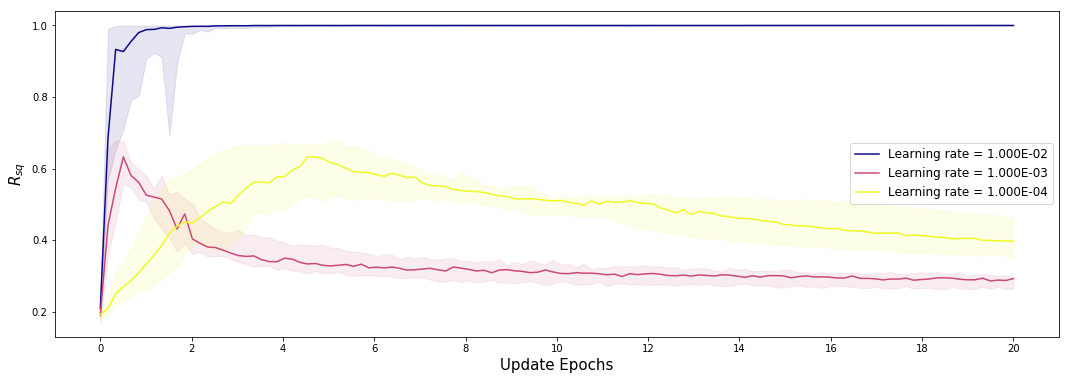
\includegraphics[width=\myWidth]{img/Sec5/sim1/dynamics_e20}
\caption[The dynamics of VNI $R_{sq}$ of the output layer.]
{
The dynamics of VNI $R_{sq}$ of the output layer.
The training is performed on the MNIST dataset 20 times, and then we evaluate the quartiles of the output VNI $R_{sq}$
for different learning rates.
Severe intensification of VNI (increases to 1 ) may occur as shown by the blue line which is trained with the learning rate of $10^{-2}$.
Otherwise VNI rises initially, and then decreases to a value which is larger than the initial VNI.
%It shows that overall, the correlation of each hidden layer is intensified during the back-propagation training. For large learning rate, the output VNI $R_{sq}$ severely increases to 1.
}
\label{fig:sec5_sim1}
\end{figure}


%%% FIGURE %%%
\begin{figure}
\centering

\newcommand{\myWidth}{0.98\linewidth}
\begin{subfigure}{\myWidth}
    \centering
    \caption{Learning rate $=10^{-3}$}
    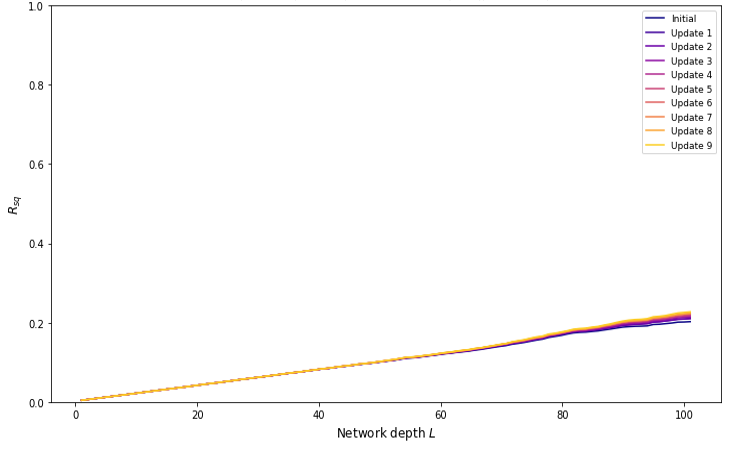
\includegraphics[width=\myWidth]{img/Sec5/sim1/Rsq_for_each_layer_0001(hard-tanh_50ave)}
    \label{fig:sec5sim15_a}
\end{subfigure}
\begin{subfigure}{\myWidth}
    \centering
    \caption{Learning rate $=10^{-2}$}
    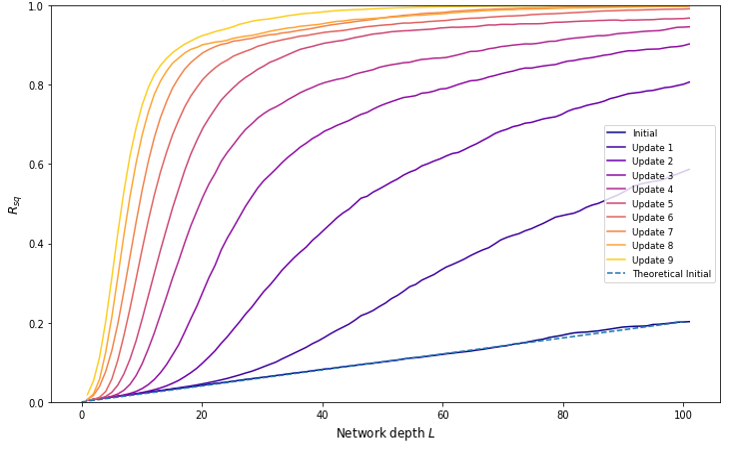
\includegraphics[width=\myWidth]{img/Sec5/sim1/Rsq_for_each_layer(hard-tanh_50ave)}
    \label{fig:sec5sim15_b}
\end{subfigure}
\caption[The dynamics of VNI $R_{sq}$ of hidden layers.]
{
    The dynamics of VNI $R_{sq}$ of hidden layers.
The training is performed on the MNIST dataset 50 times, and then we evaluate the averages of hidden layer
VNI $R_{sq}$ for learning rates $\in\{10^{-3}, 10^{-2}\}$.
%It shows that overall, the correlation of each hidden layer is intensified during the back-propagation training. For large learning rate, the output VNI $R_{sq}$ severely increases to 1.
}
\label{fig:sec5_sim15}
\end{figure}


%%% FIGURE %%%
\begin{figure}
\centering
\newcommand{\myWidth}{0.95\textwidth}
\begin{subfigure}{\myWidth}
  \centering
  \caption{Initial}
  \adjincludegraphics[width=1.0\linewidth,trim={0 0 0 0.8cm},clip]{"Hard-tanh[0]"}
  \label{fig:sec5_sim2_a}
\end{subfigure}%

\begin{subfigure}{\myWidth}
  \centering
  \caption{After 5 updates}
  \adjincludegraphics[width=1.0\linewidth,trim={0 0 0 0.8cm},clip]{"Hard-tanh[5]"}
  \label{fig:sec5_sim2_b}
\end{subfigure}%

\begin{subfigure}{\myWidth}
  \centering
  \caption{After 10 updates}
  \adjincludegraphics[width=1.0\linewidth,trim={0 0 0 0.8cm},clip]{"Hard-tanh[10]"}
  \label{fig:sec5_sim2_c}
\end{subfigure}%
\caption[The averages of squared correlation coefficients $\rho_{ij}^2$ over 50 runs.]
{The averages of squared correlation coefficients $\rho_{ij}^2$ over 50 runs.
It presents that overall, the correlation of each hidden layer are highly intensified.}
\label{fig:sec5_sim2}
\end{figure}


\section{Relationship between the VNI and the redundancy of nodes} \label{repr_redundancy}

In this section, we would like to connect the VNI $R_{sq}$ with the redundancy of nodes.
First, the $N$ random variables of node values in a hidden layer are defined as $\{X_1, X_2, ..., X_N\}$.
Without loss of generality, we assume that every $X_i$ are following $\mathcal{N}(0, 1)$ distribution.
Therefore, the covariance matrix of random vector $[X_1, X_2, ..., X_N]^T$ is
\begin{equation}
    \mathbf{C}=
    \begin{bmatrix}
        1 & \rho_{12} & \cdots & \rho_{1N} \\
        \rho_{21} & 1 & \cdots & \rho_{2N} \\
        \vdots & \vdots & \ddots & \vdots  \\
        \rho_{N1} & \rho_{N2} & \cdots & 1
    \end{bmatrix},
    \label{rv_cov}
\end{equation}
where $C_{ij}=\mathbb{E}[(X_i-\overline{X_i})(X_j-\overline{X_j})]$ as defined in
\eqref{covariance_eqn}, $\rho_{ij}$ is the correlation coefficient between $X_i$ and $X_j$,
and hence $\mathbf{C}$ is a symmetric matrix.
By the definition of the VNI $R_{sq}$ from \eqref{rsq_def}, the $R_{sq}$
can be represented as
\begin{equation}
    R_{sq}=\frac{\sum_{i=1}^N\sum_{j=1}^N\rho_{ij}^2}{N^2}
    =\frac{tr(\mathbf{C}\mathbf{C}^T)}{N^2}=\frac{1}{N^2}tr(\mathbf{C}^2).
    \label{rv_rsq}
\end{equation}
\eqref{rv_rsq}

Let the eigenvalues of $\mathbf{C}$ are $\lambda_1, \lambda_2, \dots, \lambda_N$.
By the relationship between matrix trace and eigenvalues, we have
\begin{equation}
    \begin{aligned}
        \sum_{i=1}^N\lambda_i&=tr(\mathbf{C})=N\\
    \sum_{i=1}^N\lambda_i^2&=tr(\mathbf{C}^2)=N^2R_{sq}.
    \end{aligned}
    \label{rv_eigen}
\end{equation}

To relate $R_{sq}$ with the redundancy of random variables, a method for measuring the redundancy
is needed.
From the priciple component analysis (PCA), the eigenvalue of $\mathbf{C}$ can represent the 
energy (i.e. the variance) associated with each eigenvector.
Therefore, we can use the distribution of eigenvalues $\lambda_i$ to determine the proportion of
redundant components, and hence the effective number of nodes can be evalueated.
Similar to PCA, we first rearange the order of eigenvalues $\lambda_i$ such that
$\lambda_1\geq\lambda_2\geq\cdots\geq\lambda_N\geq 0$.
We define a constant $\varepsilon\in(0, 1)$ to be the "effective threshold ratio" of eigenvalues.
That is, if $\lambda_i \geq \varepsilon\lambda_1$, then we say that the $i$-th component $\lambda_i$ is
$\varepsilon$-effective.
Otherwise, the $i$-th component $\lambda_i$ is said to be redundant.

We introduce a new metric called "$\varepsilon$-effective number of nodes ($\varepsilon$-ENN)" as
\begin{equation}
    \varepsilon\text{-ENN}
    \equiv N_{e}^\varepsilon
    \overset{\Delta}{=}max(\{t\in\mathbb{N}: \lambda_t\geq\varepsilon\lambda_1\}).
    \label{eENN_def}
\end{equation}
That is, $\varepsilon\text{-ENN}$ is the maximum number of $\varepsilon$-effective nodes.
As in \eqref{rv_eigen}, the constraints on $\lambda_i$ are already derived.
Also, it is intuitive that the maximum in \eqref{eENN_def} can simply be attained with eigenvalues
$\{\lambda_1, \varepsilon\lambda_1, \dots, \varepsilon\lambda_1, 0, \dots, 0\dots, 0\}$, where there are 
$(N_{e}^\varepsilon-1)$ $\varepsilon\lambda_1$ and $(N-N_e^\varepsilon)$ zeros.
Insert these eigenvalues into \eqref{rv_eigen}, we have
\begin{equation}
    \begin{aligned}
        \lambda_1+(N_e^\varepsilon-1)\varepsilon\lambda_1 &= N \\
        \lambda_1^2+(N_e^\varepsilon-1)(\varepsilon\lambda_1)^2 &= N^2R_{sq}.
    \end{aligned}
    \label{effective_eigen}
\end{equation}
Inserting the first equation in \eqref{effective_eigen} into the second one, we can get
\begin{equation}
    [1+(N_e^\varepsilon-1)\varepsilon]^2
    =\Big(\frac{N}{\lambda_1}\Big)
    =\frac{1+(N_e^\varepsilon-1)\varepsilon^2}{R_{sq}},
    \label{quad_eenn}
\end{equation}
which is a solvable quadratic equation. The numerical solution of the effective number of nodes for
given $\varepsilon$ are provided in Figure \ref{fig:eps_rsq}.

\begin{figure}[h]
    \centering
    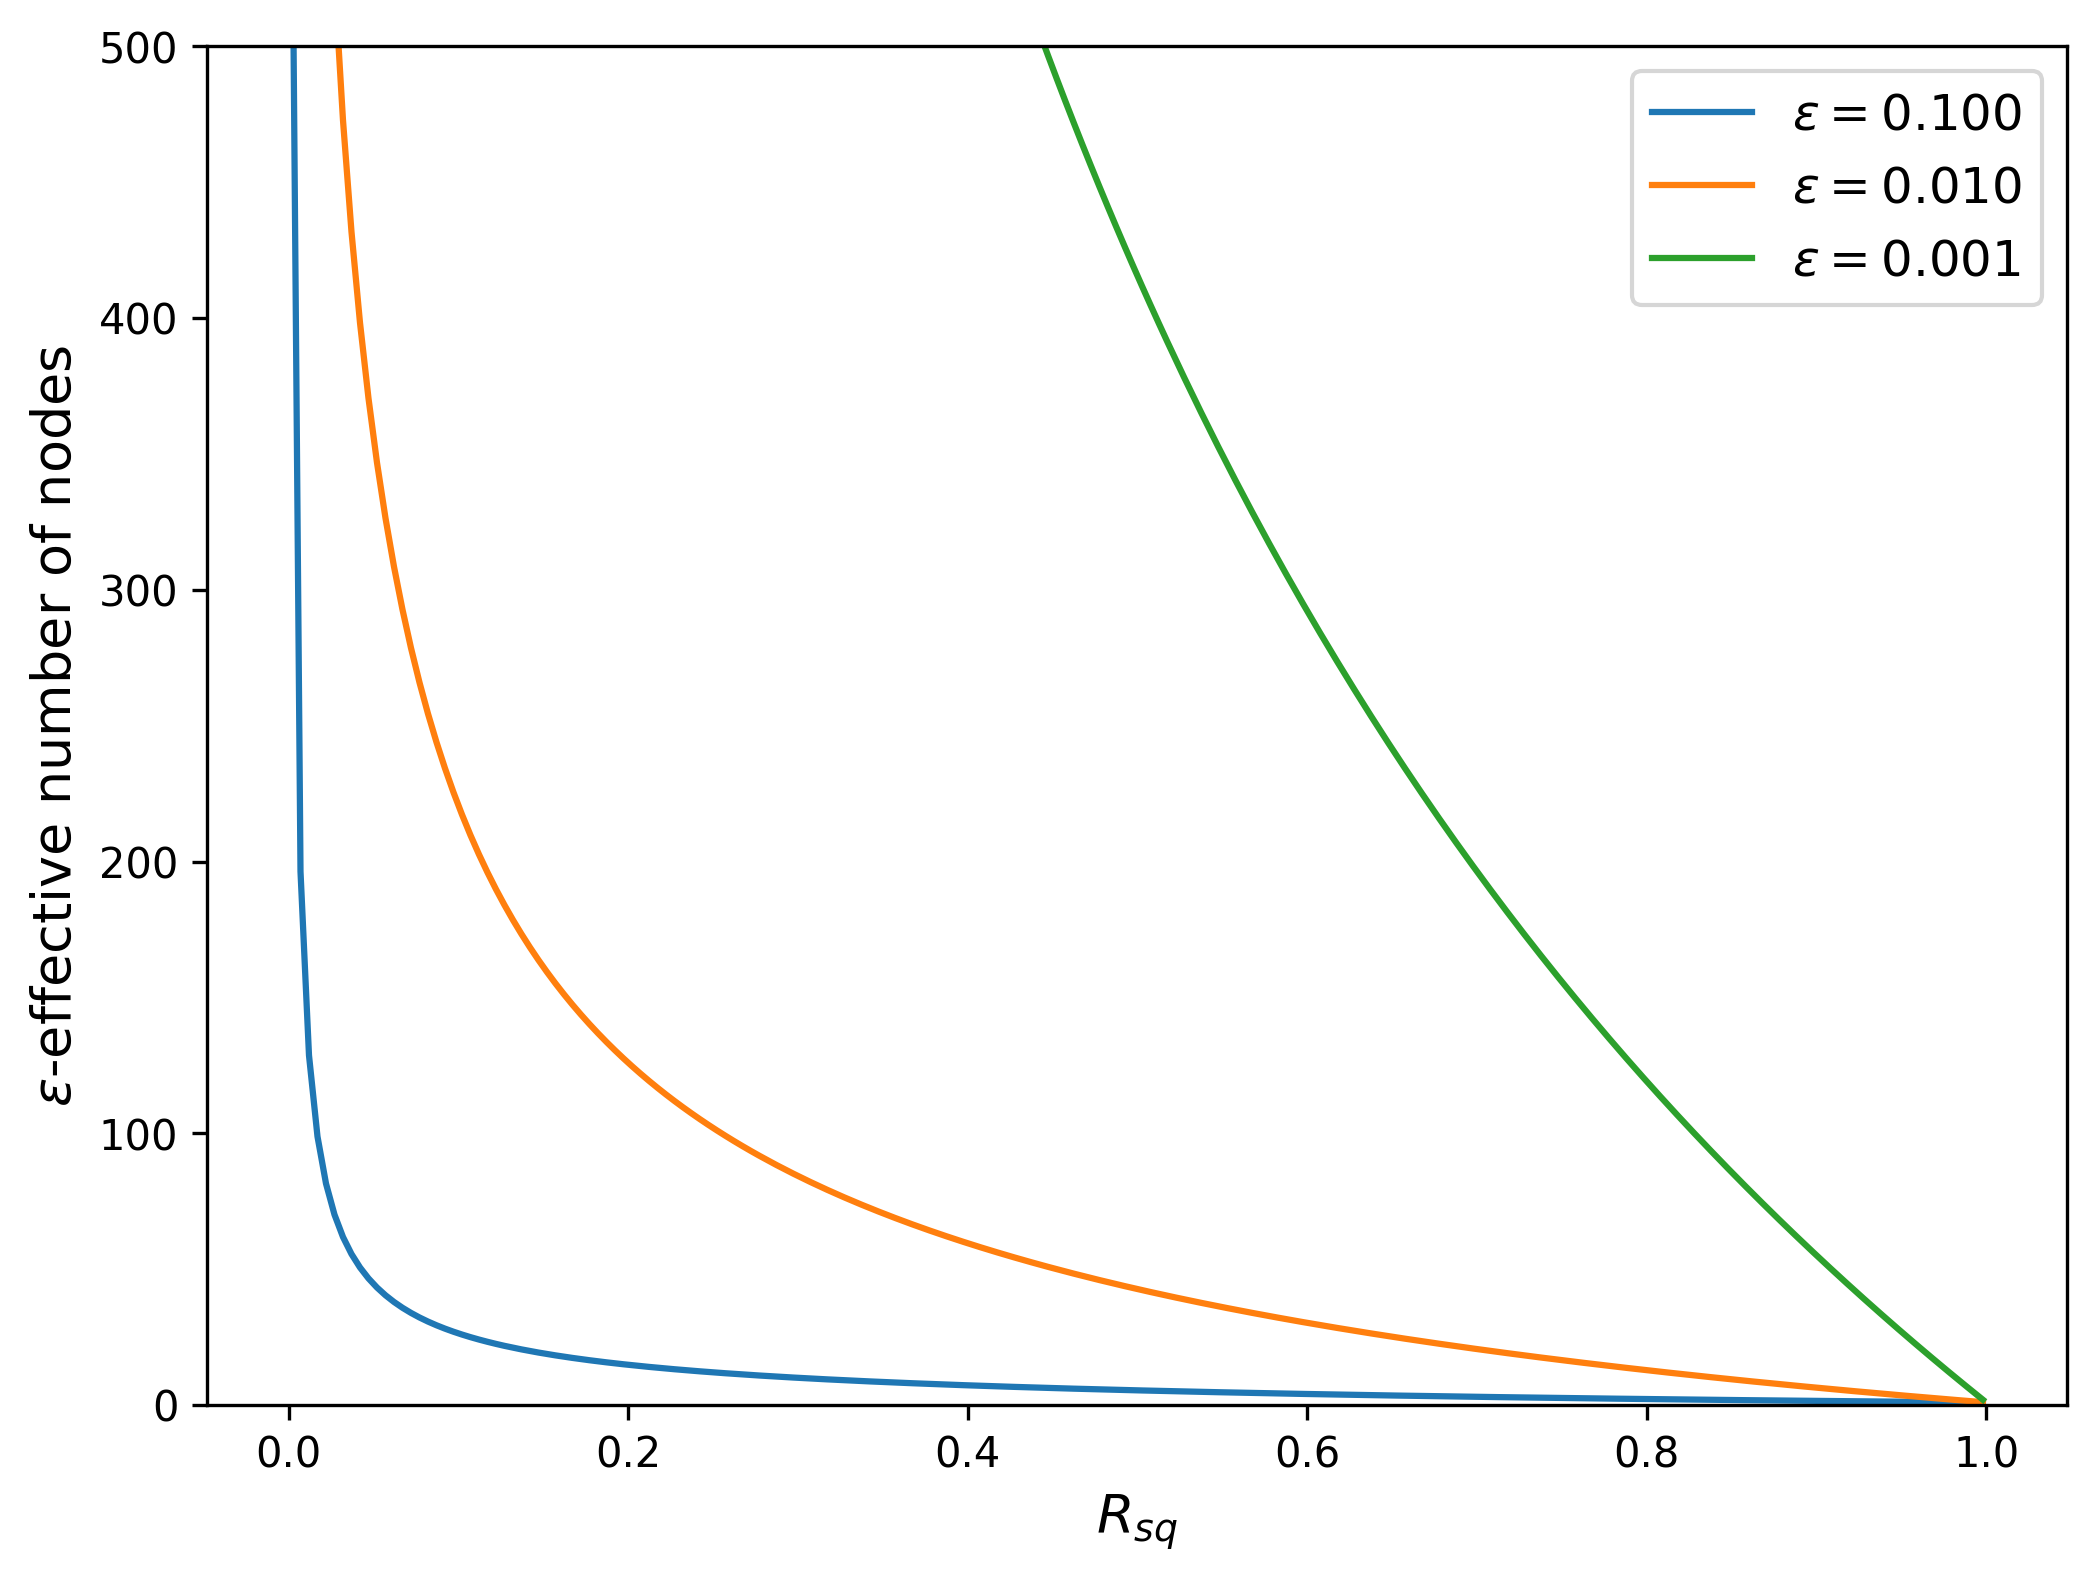
\includegraphics[width=0.9\textwidth]{eps_rsq}
    \caption[The effective number of nodes to the VNI $R_{sq}$]
    {The numerical solution of the effective number of nodes for given $\varepsilon$.
    It can be observed that the effective number of nodes vanishes as the VNI $R_{sq}$ increases to 1.
    Also, if a stricter (i.e. larger) $\varepsilon$ is chosen, the $\varepsilon$-ENN vansihes much
    faster.
    Note that the number of random variables $N$ is set to $500$.
    }
    \label{fig:eps_rsq}
\end{figure}

\begin{theorem}[Opposite trend between the VNI and the ENN]
    \label{oppo}
    For any theshold $\varepsilon$, 
    \\the $\varepsilon$-effective number of nodes strictly decreases as the VNI $R_{sq}$ increases.
\end{theorem}

\begin{proof}
        
    Evaluate the differentiation of both sides of the \eqref{quad_eenn},
    the derivative of $R_{sq}$ with respect to $N_e^\varepsilon$ is
    \begin{equation}
        \begin{aligned}
        \frac{dR_{sq}}{dN_e^\varepsilon}&=
        \frac{[1+(N_e^\varepsilon-1)\varepsilon]^2\cdot N_e^\varepsilon\varepsilon^2
        -[1+(N_e^\varepsilon-1)\varepsilon^2]\cdot N_e^\varepsilon \cdot 2\varepsilon[1+(N_e^\varepsilon-1)\varepsilon]}
        {[1+(N_e^\varepsilon-1)\varepsilon]^4}\\
        &=\varepsilon\cdot
        \frac{[1+(N_e^\varepsilon-1)\varepsilon]\cdot N_e^\varepsilon\varepsilon
        -2[1+(N_e^\varepsilon-1)\varepsilon^2]}
        {[1+(N_e^\varepsilon-1)\varepsilon]^3}\\
        &=\varepsilon\cdot
        \frac{\varepsilon-2-(N_e^\varepsilon-1)\varepsilon^2}
        {[1+(N_e^\varepsilon-1)\varepsilon]^3}\\
        &<0.
        \end{aligned}
        \label{negative_diff}
    \end{equation}

    Since in \eqref{negative_diff}, the derivative of $R_{sq}$ with respect to $N_e^\varepsilon$
    is always negative,
    the $N_e^\varepsilon$ is strictly decreasing with $R_{sq}$.

\end{proof}


\begin{theorem}[Network collapsing]
    \label{collapse}
    For any theshold $\varepsilon$,
    \\the $\varepsilon$-effective number of nodes $N_e^\varepsilon$ becomes only 1
    when the VNI $R_{sq}$ is 1.
\end{theorem}

\begin{proof}
    Insert the $R_{sq}=1$ condition into \eqref{quad_eenn}, then we have
    \begin{equation}
        \begin{aligned}
            &[1+(N_e^\varepsilon-1)\varepsilon]^2=1+(N_e^\varepsilon-1)\varepsilon^2\\
            \Rightarrow&(N_e^\varepsilon-1)[(N_e^\varepsilon-2)\varepsilon+2]=0\\
            \Rightarrow& N_e^\varepsilon=1
        \end{aligned}
        \label{collapse_eqn}
    \end{equation}

    The solution of $N_e^\varepsilon$ in \eqref{quad_eenn} is $1$ 
    (no matter the value of $\varepsilon$).
    Therefore, the $\varepsilon$-effective number of nodes $N_e^\varepsilon$ becomes only 1
    when the VNI $R_{sq}$ is 1.
\end{proof}

By Theorem \ref{oppo}, and Theorem \ref{collapse}, we can say that the effective number of nodes
in a layer of a network vanishes to 1 as the VNI $R_{sq}$ increases to 1.
If the output layer
of a network has the VNI $R_{sq}=1$, then we can say that the network suffers from the
"\textit{network collapsing}" problem, which has only 1 effective node at the output layer and
hence cannot solve most of training tasks.
% In Section \ref{repr_general}, we will show that the VNI $R_{sq}$ will increase to 1 when the depth of the network goes large enough.

\iffalse
In probability theory and in particular in information theory, \textit{total correlation}
(\cite{total_corr}) is one of metric used to quantify the redundancy among random variables.
The definition of total correlation ($TC$) is defined as the Kullback–Leibler divergence (\cite{KL_div})
from the joint distribution to the independent distribution of $\{X_1, X_2, \dots, X_N\}$. That is,
\begin{equation}
    TC\overset{\Delta}{=}D_{KL}[p(X_1, \dots, X_N)||p(X_1)p(X_2)\cdots p(X_N)],
    \label{def_total_corr}
\end{equation}
where $D_{KL}$ is the Kullback–Leibler divergence, $p(X_1, \dots, X_N)$ is the joint distribution and
$p(X_1)p(X_2)\cdots p(X_N)$ is the independent distribution of $\{X_1, X_2, \dots, X_N\}$.
Note that the range of $TC$ is $[0,\infty)$, and the higher value representation the 

The definition of the Kullback–Leibler divergence is
\begin{equation}
    D_{KL}(P||Q)=\int_{-\infty}^{\infty}p(x)log\Big(\frac{p(x)}{q(x)}\Big)dx.
    \label{def_kl}
\end{equation}
Also, the probability density functions of normal distribution are
\begin{equation}
    \begin{aligned}
        (\forall i), \;p(X_i) &= \frac{1}{\sqrt{2\pi}}exp\Big(-\frac{x^2}{2}\Big)\\
        p(X_1, \dots, X_N)&=\frac{1}{\sqrt{(2\pi)^N|\mathbf{C}|}}
            exp\Big(-\frac{1}{2}\mathbf{x}^T\mathbf{C}^{-1}\mathbf{x}\Big).
    \end{aligned}
    \label{def_normal}
\end{equation}
From \eqref{def_kl} and \eqref{def_normal}, the Kullback–Leibler divergence between two normal
distribution $P$ and $Q$ is
\begin{equation}
    \begin{aligned}
        D(P||Q)&=\mathbb{E}_P[log(P)-log(Q)]\\
        &=\frac{1}{2}\mathbb{E}_P[-log(|\mathbf{C}_P|)-\mathbf{x}^T\mathbf{C}_P^{-1}\mathbf{x}
        +log(|\mathbf{C}_Q|)-\mathbf{x}^T\mathbf{C}_Q^{-1}\mathbf{x}]\\
        &=\frac{1}{2}log\Big(\frac{|\mathbf{C}_Q|}{|\mathbf{C}_P|}\Big)
        +\frac{1}{2}\mathbb{E}_P[-tr(\mathbf{C}_P^{-1}\mathbf{C}_P)
        +tr(\mathbf{C}_Q^{-1}\mathbf{xx}^T)]\\
        &=\frac{1}{2}log\Big(\frac{|\mathbf{C}_Q|}{|\mathbf{C}_P|}\Big)-N+
        tr(\mathbf{C}_Q^{-1}\mathbf{C}_P),
    \end{aligned}
    \label{kl_normal}
\end{equation}
where $|\mathbf{C}|\equiv det(\mathbf{C})$ is the determinant of $\mathbf{C}$.

Therefore, the total correlation of $\{X_1, X_2, \dots, X_N\}$ is
\begin{equation}
    \begin{aligned}
        TC&=D_{KL}[p(X_1, \dots, X_N)||p(X_1)p(X_2)\cdots p(X_N)]\\
        &=\frac{1}{2}log\Big(\frac{|I|}{|\mathbf{C}|}\Big)-N+
        tr(\mathbf{C})\\
        &=-\frac{1}{2}log(|\mathbf{C}|)\\
        &=-\frac{1}{2}\sum_{i=1}^Nlog(\lambda_i).
    \end{aligned}
    \label{kl_derive}
\end{equation}
Note that in \eqref{kl_derive} we use the fact that the determinant of a matrix is equal to the
product of all eigenvalues.

\fi


\section{The vanishing of the representation power} \label{repr_general}

The phenomena that the representation power of a very deep network vanishes
is shown in this section.
Recent works \cite{mft:expo, expressive, linear_regions, expr_power, relu_understand,
relu_benifit, relu_approx} put emphasis on the benifit of increasing the depth of a neural network,
and claim that the representation power of a neural network grows exponentially as its depth. 
However, the representation power discussed in previous results is mainly the theoretical upper bound of
all variable space.
Practically, it has small probability for the representation power to reach the upper bound when
the weight matrices are randomly initialized.
In the following, we will show that if the weight matrices are drawn from a non-orthogonal
probability distribution (such as the normal distribution and the uniform distribution), the VNI
$R_{sq}$ increases to 1 as the network goes deeper. Moreover, as the VNI $R_{sq}$ reaches nearly 1,
the representation power of the network will vanish.

The VNI $R_{sq}$ has been defined in \eqref{rsq_def} to measure the correlation between the output nodes of
a network, and hence the VNI can be viewed as a measurement of the level of redundancy.
In Section \ref{repr_redundancy}, the redundant number of nodes has already been connected to the
VNI $R_{sq}$. Therefore, we can simply use the VNI $R_{sq}$ as an approximation of the ratio of redunt
nodes, and the number of effective nodes can be approximated as $N\cdot(1-R_{sq})+1$, that is,
one node along with other non-redundant nodes.
Because the representation power is closely related to the effective number of network nodes, the VNI
$R_{sq}$ can provide an estimation of the representation power.
 
In Figure \ref{fig:repr_general}, the network width $N$ is set to $500$ and the network depth
$L$ ranges from $1$ to $10000$. The network is fed with 1000 randomly generated data point
drawn from zero-mean white Gaussian distribution with standard deviation equals to $0.1$.
The VNI $R_{sq}$ are evaluated according to the definition in \eqref{rsq_def}.
The weights are initialized with scaled-Gaussian distribution (\cite{xavier, he}), which
will be discussed in Section \ref{comp:init}, and the biases are initialized to zeros.
The activation functions of the networks include tanh, ReLU and linear. Note that for the
ReLU case, we add the layer normalization (\cite{layer_norm}) blocks between hidden layers
in order to prevent the node values from converging to zeros. If the node values converges
to zeros, the result of \eqref{rsq_def} become undefined.
Also note that since in our case, the layer
normalization only rescale the node values, it will not affect the value of VNI evaluated
from \eqref{rsq_def}, which is a scale-invariant metric.
The simulation is repeated for 20 times, and the medians of the VNI over 20 runs are plotted as
the solid lines, and the boundaries of the colored regions are the first and the third
quartiles of the VNI. It is shown that for a feed-forward architecture under a non-orthogonal
initialization, the initial VNI $R_{sq}$ increases to 1 as $L$ gets larger. That is,
the representation power vanishes as the network goes deeper. The VNI of ReLU activation,
especially, grows in the steepest with the network depth, and the reason can be observed from
the \eqref{rsq_moment}, Table \ref{table:mu} and Table \ref{table:s}. The $R_{sq}$ 
approximated by \eqref{rsq_moment} for ReLU activation is $(2L+1)/N$ while the $R_{sq}$
for linear and tanh activation is nearly $(L+1)/N$.
Therefore, the ReLU activation suffers more from the vanishing representation power.

We define the "maximal depth" as the maximal $L$ such that in less than half of 20
runs(i.e. 10 runs), the approximated number of effective nodes achieve greater than 1.
The maximal depths for different activation functions, weight initializations and network
architectures are shown in Table \ref{dead_table}. It shows that the maximal depth of ReLU
activation is much less than linear and tanh activations. It has been stated
\cite{relu_sparse} that the ReLU activation provides a sparse and distributed representation
That is, the ReLU activation selects half of neurons as the active nodes, which may reduce the
effective number of nodes. Since the maximal depth is closely related to the effective number
of nodes, it provide another aspect explaining that the representation power vansihes
faster for the ReLU activation.

Here, we provide a theoretical claim for reasoning the VNI $R_{sq}$ of a Gaussian initialized
linear network.

\begin{theorem}[The VNI $R_{sq}$ goes to 1 as $L\rightarrow\infty$]
    For a linear network with Gaussian initialized weight matrices
    $\mathbf{W}_l, l\in\{1, 2, \dots, L\}$, the VNI $R_{sq}$ of
    the network goes to 1 as $L\rightarrow\infty$.
    \label{matrix_prod}
\end{theorem}

\begin{proof}
    Let the product of weight matrices $\mathbf{P}$ as the input-output Jacobian
    (defined in \eqref{jacobian_eqn}) of the linear network
    \begin{equation}
        \mathbf{P}_L\equiv\prod_{l=1}^L\mathbf{W}_l.
        \label{prod_def}
    \end{equation}
    From \eqref{rsq_eigen}, we would like to show that
    $R_{sq}=\frac{\sum_{k=1}^N\lambda_k^2}{(\sum_{k=1}^N\lambda_k)^2}$
    goes to 1 as $L\rightarrow\infty$.
    Note that the $\lambda_k$ is the $k$-th eigenvalue of $\mathbf{P}_L\mathbf{P}_L^T$, satisfying
    $\lambda_1\leq\lambda_2\leq\dots\leq\lambda_N$.

    Considering the asymptotic behavior of eigenvalues $\lambda_k$ when the depth $L$ tends to
    infinity,
    we can apply the Lyapunov exponents to the matrix $\mathbf{P}_L\mathbf{P}_L^T$ as
    in \cite{prod_mat}.
    \begin{equation}
        \lim_{L\rightarrow\infty}(\mathbf{P}_L\mathbf{P}_L^T)^{1/2L}=e^\mathbf{H},
        \label{lyap_exp}
    \end{equation}
    where $\mathbf{H}$ has eigenvalues $\mu_1\leq\mu_2\leq\dots\leq\mu_N$, which are known as the
    Lyapunov exponents.

    By the Oseledec's theorem \cite{osel_thm}, we have the asymptotic value of eigenvalue
    \begin{equation}
        \lambda_k\sim e^{2L\mu_k}.
        \label{asym_eig}
    \end{equation}
    Previous works (\cite{prod_mat}) have already derived the value of $\mu_k$
    \begin{equation}
        \mu_k=\frac{1}{2}\log 2 + \frac{1}{2}\psi\Big(\frac{k}{2}\Big),
        \label{mu_result}
    \end{equation}
    where $\psi(\cdot)$ denotes the \textit{digamma function}, which is defined as the logarithmic
    derivative of the gamma function.
    As in \cite{digamma}, the digamma function has the asymptotic expansion
    \begin{equation}
        \psi(x)\sim\log x-\frac{1}{2x}+O(x^{-2}).
        \label{digamma_asym}
    \end{equation}

    Therefore, the eigenvalues $\lambda_k$ has the asymptotic approximation by \eqref{asym_eig} to
    \eqref{digamma_asym}
    \begin{equation}
        \lambda_k\sim e^{L(\log k)}=k^L.
        \label{eig_approx}
    \end{equation}
    Insert the result of \eqref{eig_approx} into \eqref{rsq_eigen}, we have
    \begin{equation}
        \begin{aligned}
        \lim_{L\rightarrow\infty}\frac{\sum_{k=1}^N \lambda_k^2}{\big(\sum_{k=1}^N \lambda_k\big)^2}
        &=\lim_{L\rightarrow\infty}\frac{\sum_{k=1}^N k^{2L}}{\big(\sum_{k=1}^N k^L\big)^2}\\
        &=\lim_{L\rightarrow\infty}\frac{\sum_{k=1}^N (k/N)^{2L}}{\big(\sum_{k=1}^N (k/N)^L\big)^2}\\
        &=1.
        \end{aligned}
        \label{eig_result}
    \end{equation}

    That is, the VNI $R_{sq}$ of
    a linear network with Gaussian initialized weight matrices goes to 1 as $L\rightarrow\infty$.

\end{proof}

%, since the \textit{width} of a neural network also matters.
%According to the "universal approximation theorem" proved by \cite{universal}, a single hidden layer with a finite number of neurons can approximate continuous functions on compact subsets.
%That is, the number of neurons in a network is closely related to its representation power, which is .

%Vanishing node is a problem that in some cases, several nodes in hidden layers or the output layer in a neural network architecture are highly correlated even if nodes of the input layer are independent.
%Correlations imply dependencies, and dependencies produce redundancy.
%That is, in the worst case, all of hidden nodes or output nodes are so correlated that if we remove the redundant nodes, the number of remaining nodes are much less than the original network width.
%Therefore, we name this phenomena as the \textit{vanishing node problem}.

\section{The effect of the orthogonal weight matrices to the representation power} \label{repr_orthogonal}

The orthogonal weight initialization \cite{mft:linear} is one of methods that train a very
deep neural network successfully. In \cite{mft:cnn}, the trainable depth of a convolutional
neural network with orthogonal initialized weights can reach over 10000 layers. In this
section, we will show that the orthogonal weight matrices can prevent the representation
power of networks from vanishing.

In Figure \ref{fig:repr_orthogonal}, similar settings to Figure \ref{fig:repr_general} are 
used excluding the weights, which are initialized with scaled-Orthogonal distribution
(\cite{mft:linear}, further discussion is provided in Section \ref{comp:init}). It is shown
that for a feed-forward architecture under the orthogonal initialization with linear or tanh
activation function, the initial VNI $R_{sq}$ remain nearly
minimum (1/N) even when the network depth $L$ gets larger, and that the VNI of ReLU
activation increases to 1 as the network goes deeper.

From \eqref{rsq_moment} and Table \ref{table:s}, it can be derived that the approximation of
the VNI $R_{sq}$ of networks with orthogonal weight matrices is 
$\Big[\Big(\frac{\mu_2}{\mu_1^2}-1\Big)L+1\Big]\Big/N$. That is, if an activation function
such that $\frac{\mu_2}{\mu_1^2}\sim1$ is chosen, then the VNI $R_{sq}$ can remain
in a lower level even when the network goes much deeper. Therefore, it explains that the 
network with linear and tanh activation has a constant VNI $R_{sq}$ with respect to the
network depth, and the VNI $R_{sq}$ for the network with ReLU activation still increases
to 1.

To provide a more intuitive explanation, we first consider the linear activation case.
Because the product of orthogonal matrices remain an orthogonal matrix, the input-output
correlation for a 10000-layer network with orthogonal weights can be reduced to a 1-layer
shallow network with a single orthogonal weight. Therefore for such a network setting, the
representation power remain the same even if the network depth $L$ goes arbitrarily large.

Consider the ReLU activation network with orthogonal weight matrices. The output layer is
$\mathbf{x}_L=\phi(\mathbf{W}_L\dots\phi(\mathbf{W}_2\phi(\mathbf{W}_1\mathbf{x}_0)))$.
Analytically, the ReLU activation function $\phi(\cdot)$ can be taken as a matrix
$\mathbf{U}_l$ with all the off-diagonal elements equal to zeros and the diagonal elements
$\in\{0, 1\}$, which are dependent to the input data. That is, the output layer can be
expressed as
$\mathbf{x}_L=(\mathbf{U}_L\mathbf{W}_L)\dots(\mathbf{U}_2\mathbf{W}_2)(\mathbf{U}_1\mathbf{W}_1)\mathbf{x}_0$.
Note that the matrices $(\mathbf{U}_l\mathbf{W}_l)$ can be viewed as the random samples
from the row vectors of the orthogonal matrix $\mathbf{W}_l$.
Since the random sample operation is equivalent to the random projection onto the coordinate
hyperplanes, the orthogonal property of $\mathbf{W}_l$ will be no longer kept after the
multiplication with $\mathbf{U}_l$.
Therefore, the representation power of the network faced the same problem as stated in
Section \ref{repr_general}.

The maximal depths for different activation functions with orthogonal weight initializations
are also shown in Table \ref{dead_table}. It shows that the maximal depths of linear and tanh
activations are more than 10000 layers, but that of ReLU activation is much small, which is
consistent to our analysis.

\section{Representation power of residual-like architectures} \label{repr_residual}

Residual network (\cite{resnet1, resnet2}) is another example for training very deep nerual
networks successfully.
Unlike the orthogonal weight initialization, the residual network is one of an architecture
solution to improve the training performance. In this section, the advantage of the 
additional identity skip connections (i.e. residual shortcut connections) and the effect
to the representation power will be discussed.

First, the network architecture to be considered is present in Figure \ref{fig:resnet_def}, which is
similar to \cite{resnet2}. For the 1-layer shortcut case in Figure \ref{fig:resnet_def1}, we can
rewrite the network equation defined in \eqref{network_eqn} as
\begin{equation}
    \begin{aligned}
        \mathbf{x}_{l}&=\mathbf{x}_{l-1} + \mathcal{F}(\mathbf{W}_l, \mathbf{x}_{l-1})\\
        &=\mathbf{x}_{0} + \sum_{i=0}^{l-1}\mathcal{F}(\mathbf{W}_{i+1}, \mathbf{x}_{i}),
    \end{aligned}
\label{resnet_eqn}
\end{equation}
where $\mathcal{F}(\cdot)$ is the residual block function consist of batch normalization
(\cite{batchnorm}), activation function and weight multiplication.
After the first-order approximation as \eqref{covariance_eqn}, the residual block function
$\mathcal{F}(\mathbf{W}_l, \mathbf{x}_{l-1})$ can be approximated as $\mathbf{F}_l\mathbf{x}_{l-1}$.
Therefore, the input-output Jacobian matrix $\mathbf{J}$ can be expressed as
$\prod_{l=1}^{L}(\mathbf{I}+\mathbf{F}_l)$, where $\mathbf{I}$ is the identity matrix.
The whole network hence can be viewed as a feed-forward network with weight matrices
$\widehat{\mathbf{F}_l}\equiv(\mathbf{I}+\mathbf{F}_l)$. 

We would like to show that the increasing effect to the VNI $R_{sq}$ 
of $\widehat{\mathbf{F}_l}$ is much less than that of $\mathbf{F}_l$
by comparing the expected cosine similarity between column vectors of 
$\widehat{\mathbf{F}_l}$ and $\mathbf{F}_l$.
Since the hidden nodes of $\mathbf{x}_l$ can be approximated as a result of linear transformation of
$\mathbf{x}_{l-1}$ with column vectors of $\widehat{\mathbf{F}_l}$ or $\mathbf{F}_l$,
the VNI $R_{sq}$ of layer $l$, which is the weighted average of correlation coefficient of
$\mathbf{x}_l$, is highly dependent on the magnitude of the cosine similarity between column vectors
of the transformation matrix.

First, the cosine similarity between two vectors is defined as
\begin{equation}
    cos(\mathbf{a}, \mathbf{b}) \overset{\Delta}{=}
    \frac{\mathbf{a}^T\mathbf{b}}{||\mathbf{a}||\cdot||\mathbf{b}||},
    \label{def_cosine}
\end{equation}
where $||\mathbf{v}||$ denotes the $L_2$-norm of vector $\mathbf{v}$
(i.e. $\sqrt{\mathbf{v}^T\mathbf{v}}$).
Note that the transformation matrix $\mathbf{F}_l$ is basically the product of $\mathbf{D}_l$
(defined in \eqref{jacobian_eqn}) and $\mathbf{W}_l$, and therefore the $\mathbf{F}_l$ inherits
the zero-mean property of $\mathbf{W}_l$.
Let the $i$-th column vectors of $\widehat{\mathbf{F}_l}$ and $\mathbf{F}_l$ be written as
$\widehat{\mathbf{f}}_{l(i)}$ and $\mathbf{f}_{l(i)}$.
By the fact that $\widehat{\mathbf{F}_l}\equiv(\mathbf{I}+\mathbf{F}_l)$, we have
\begin{equation}
    \begin{aligned}
    \widehat{\mathbf{f}}_{l(i)}
    &=\mathbf{f}_{l(i)}+[\underset{(i-1)}{0, \dots, 0}, 1, \underset{(N-i)}{0, \dots, 0}]^T\\
    &=[f_{l(i,1)},\dots,f_{l(i,i-1)},(f_{l(i,i)}+1),f_{l(i,i+1)},\dots,f_{l(i,N)}]^T.
    \end{aligned}
    \label{hat_iden_add}
\end{equation}

Therefore, the cosine similarity between $i$-th and $j$-th column vectors of
$\widehat{\mathbf{F}_l}$ can be expressed as
\begin{equation}
    \begin{aligned}
        cos(\widehat{\mathbf{f}}_{l(i)}, \widehat{\mathbf{f}}_{l(j)})
        &\equiv\frac
        {\widehat{\mathbf{f}}_{l(i)}^T\widehat{\mathbf{f}}_{l(j)}}
        {||\widehat{\mathbf{f}}_{l(i)}||\cdot||\widehat{\mathbf{f}}_{l(j)}||}\\
        &=\frac
        {\mathbf{f}_{l(i)}^T\mathbf{f}_{l(j)}+f_{l(i,j)}+f_{l(j,i)}}
        {\sqrt{||\mathbf{f}_{l(i)}||^2+2f_{l(i,i)}+1}\cdot\sqrt{||\mathbf{f}_{l(j)}||^2+2f_{l(j,j)}+1}},
    \end{aligned}
    \label{res_cosine}
\end{equation}
which has a smaller magnitude (compared with $cos(\mathbf{f}_{l(i)}, \mathbf{f}_{l(j)})$) with high
probability (as shown in Figure \ref{cosine_comp}).
That is, the residual-like transfromation is closer to the orthogonality than the vanilla
feed-forward transformation.

\begin{figure}[h]
    \centering
    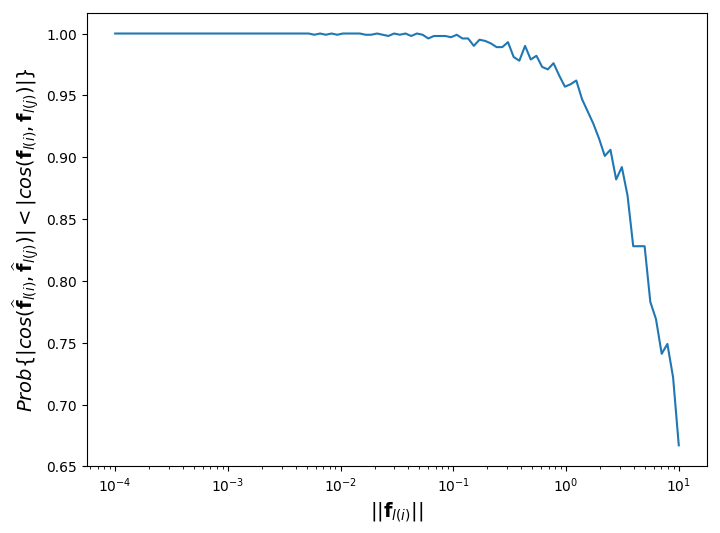
\includegraphics[width=0.9\textwidth]{cos_comp}
    \caption[Numerical simulation for \eqref{res_cosine}]
    {The probability of 
    $|cos(\widehat{\mathbf{f}}_{l(i)}, \widehat{\mathbf{f}}_{l(j)})|<|cos(\mathbf{f}_{l(i)}, \mathbf{f}_{l(j)})|$
    is shown in this figure.
    The simulation is performed with 1000 pairs of random vectors drawn from zero-mean white Gaussian
    for every $||\mathbf{f}_{l(i)}||$.
    The network width $N$ is set to 500.
    Note that practically, $||\mathbf{f}_{l(i)}||$ is much smaller than $1$ because the 
    normalization operation (e.g. batch normalization \cite{batchnorm}) included in $\mathbf{F}_l$
    will reduce the magnitude of nodes for the residual network.
    It shows that with high probability, the residual-like transfromation is closer to the
    orthogonality than the vanilla feed-forward transformation.}
    \label{cosine_comp}
\end{figure}

That is, compared with the original feed-forward network with the layer-by-layer transformation
$\mathbf{F}_l$, the residual-like architecture with identity shortcut connection has the
layer-by-layer transformation $\widehat{\mathbf{F}_l}=\mathbf{I}+\mathbf{F}_l$,
which is more close to the orthogonality even when the activation funciton is ReLU.
From the results of Section \ref{repr_orthogonal}, we can say that the residual-like architecture
suffer less from the vanishing representation power problem.

In Figure \ref{fig:repr_residual}, similar settings to Figure \ref{fig:repr_general} are 
used excluding the network architectures, which are defined in Figure \ref{fig:resnet_def}.
It is shown that for a residual-like architecture, the VNI $R_{sq}$ grows slowly as the network
depth $L$ gets larger. The ReLU activation function, which results in the vanishing representation
power in Section \ref{repr_general} and \ref{repr_orthogonal}, does not make the VNI $R_{sq}$ go
to 1 in 10000 layers. Instead, the VNI $R_{sq}$ for a 10000-layer residual ReLU network grows to a
relatively small value ($\sim0.04$), which implies that the network maintains enough representation
power even when the network is very deep.
Also, the VNI $R_{sq}$ for the 2-layer skip grows more slowly than that for the 1-layer skip. It 
can be reasoned that the 2-layer skip architecture, in some sense, reduces the effective network depth
to nearly $L/2$ because the input-output Jacobian for the 2-layer skip architecture can be
expressed as $\prod_{i=1}^{L/2}(\mathbf{I}+\mathbf{F}_{2i-1}\mathbf{F}_{2i})$.

The maximal depths of residual-like network for different activation functions with scaled-Gaussian
weight initialization are also shown in Table \ref{dead_table}.
It shows that no matter which activation function is chosen, the maximal depths of the networks are
more than 10000 layers. That is, the residual-like architecture can prevent the network representation
power from intensely vanishing. Similar results can be observed in Figure \ref{fig:repr_architecture}.

Also, in Figure \ref{fig:repr_cnn}, we perform the simulation on convolutional neural networks.
The feature sizes of hidden layers are all the same (32 width, 32 height and 5 channels), and the
network is fed with 1000 randomly generated image following the zero-mean white Gaussian.
The stride and the dilation are set to 1, and pooling layers are not inserted into the network.
The VNI $R_{sq}$ is evaluated with flatten vectors.
The median, the first and third quartiles of VNI $R_{sq}$ over 20 runs are presented.
It shows that the convolution operation can make the VNI $R_{sq}$ increase slower with respect to
the network depth $L$, and similar to Figure \ref{fig:repr_architecture}, the residual connection
helps the network maintain the representation power.

\begin{figure}[h]
    \centering
    \newcommand{\myWidth}{0.9\textwidth}
    \begin{subfigure}{\myWidth}
      \centering
      \caption{Network depth $L\in[1, 10000]$}
      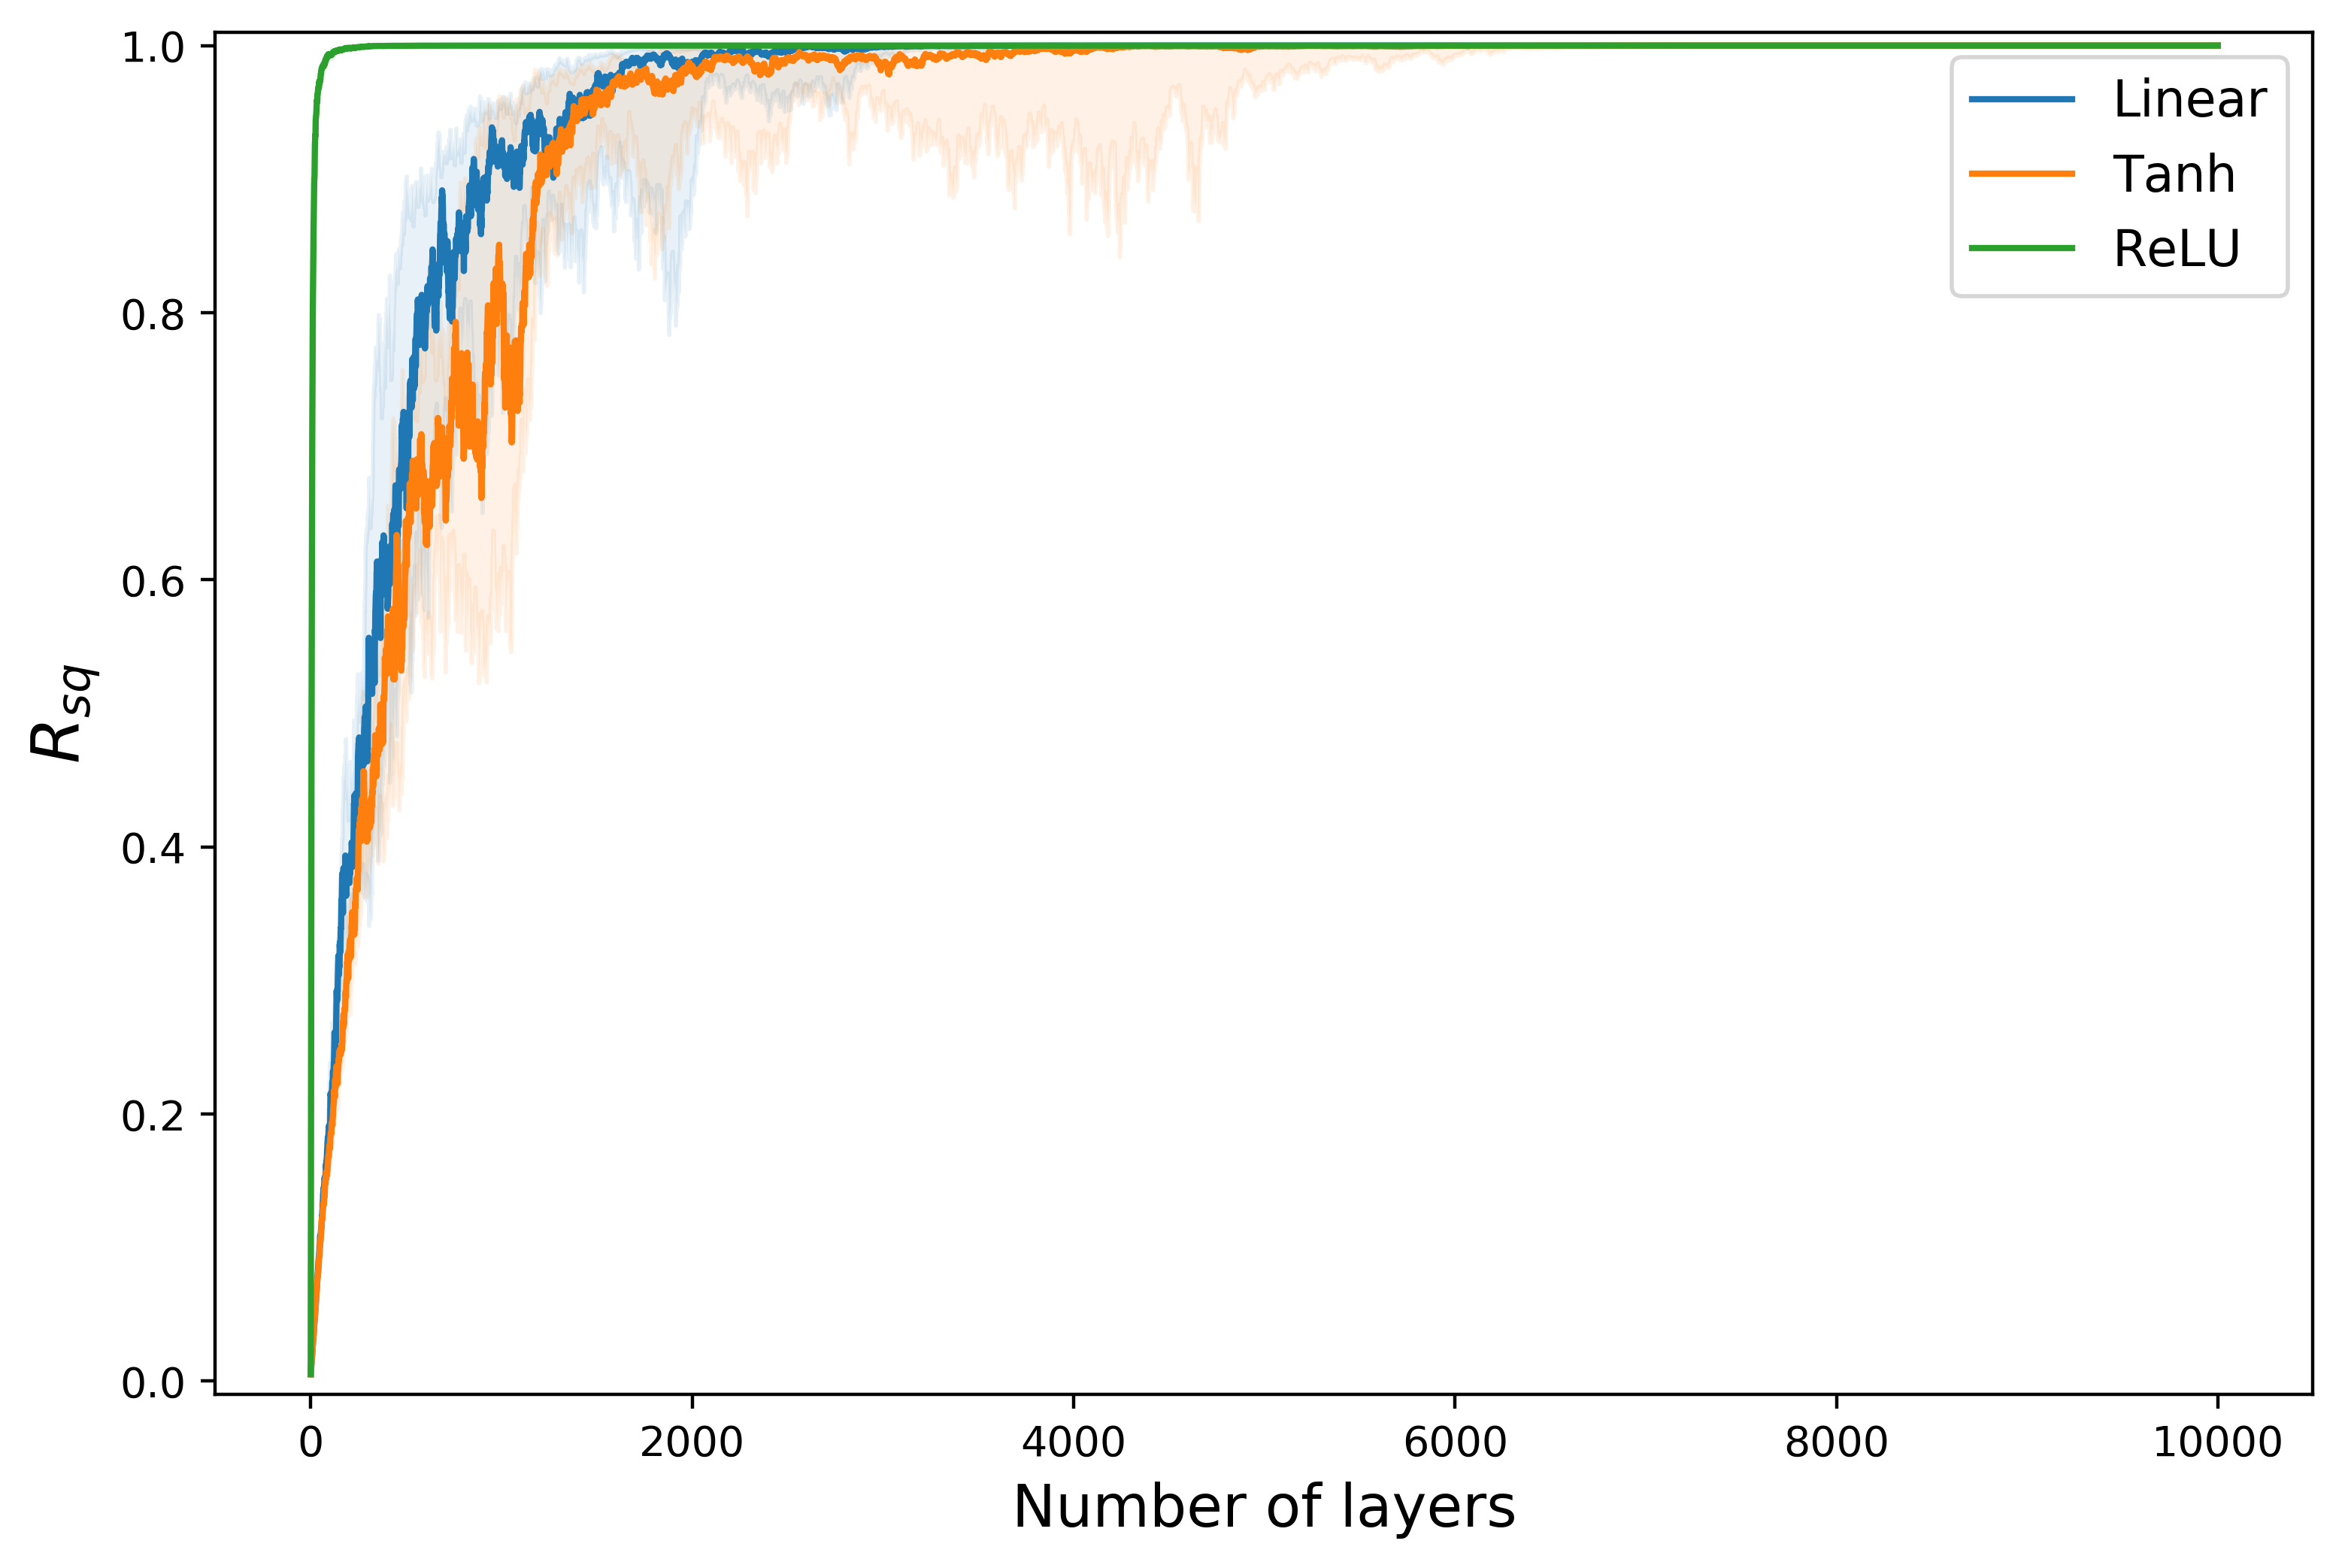
\includegraphics[width=1.0\linewidth]{10000_layer_rsq}
      \label{fig:repr_general_a}
    \end{subfigure}
    
    \begin{subfigure}{\myWidth}
      \centering
      \caption{Network depth $L\in[1, 500]$}
      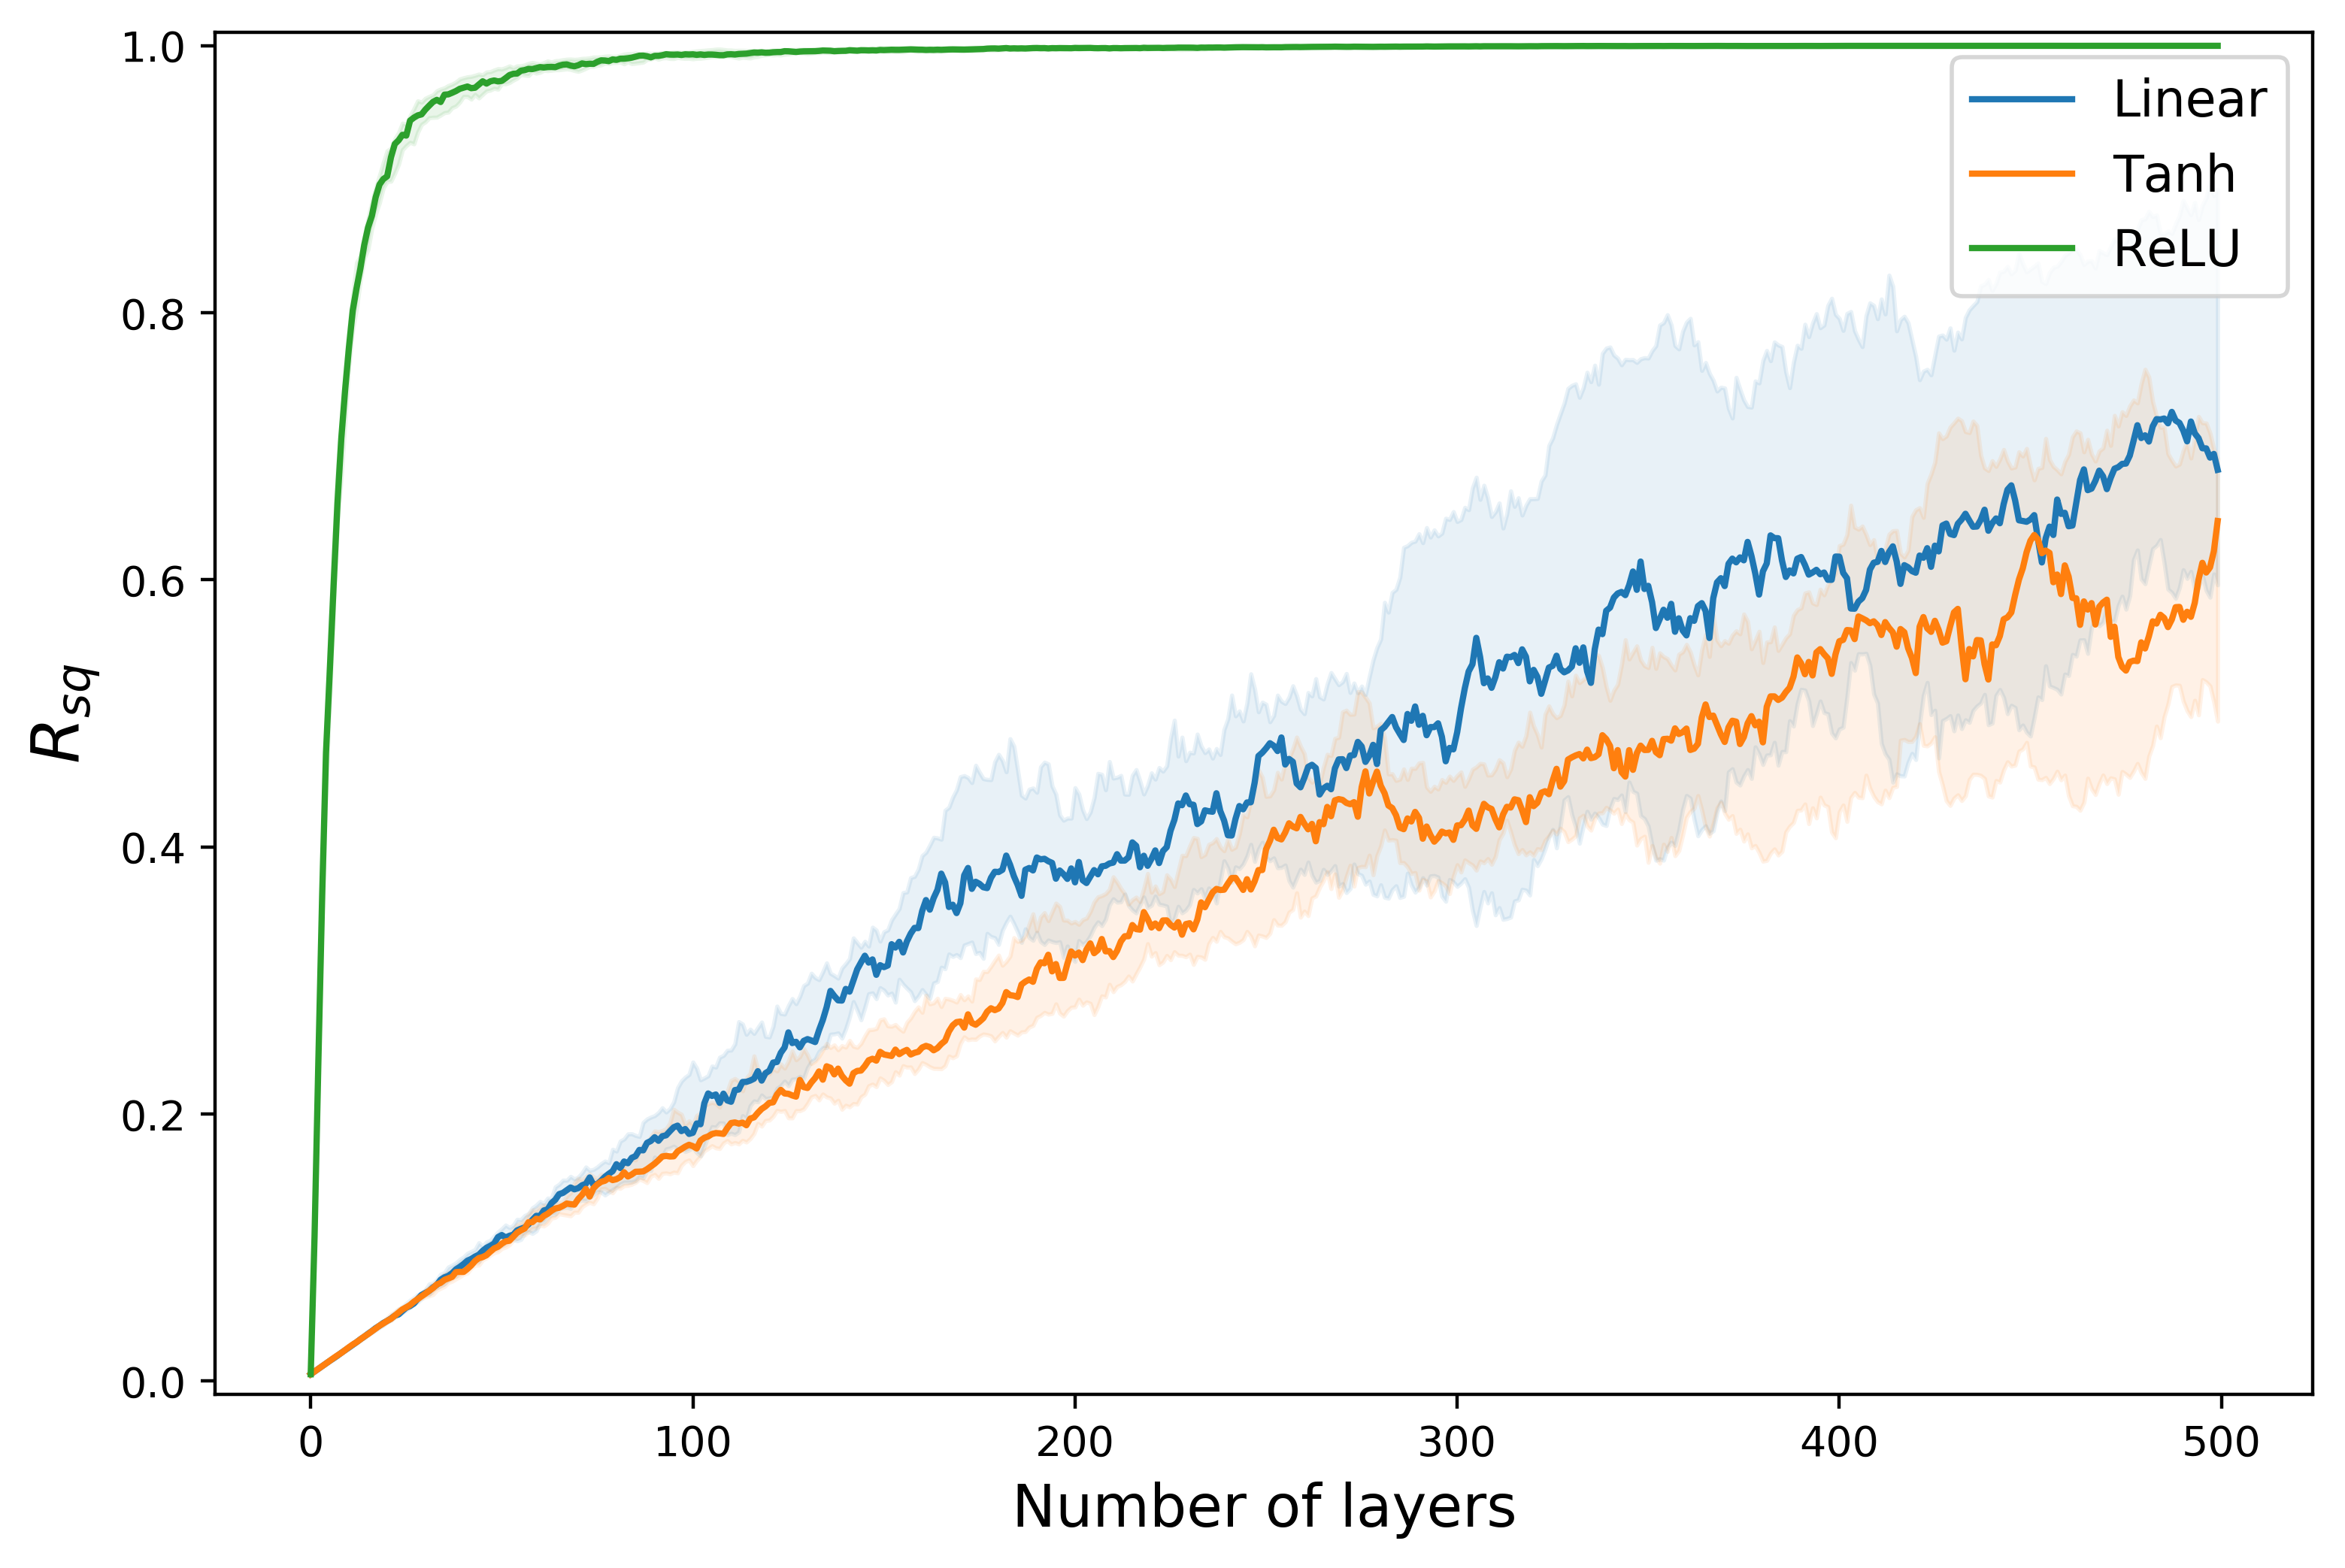
\includegraphics[width=1.0\linewidth]{500_layer_rsq}
      \label{fig:repr_general_b}
    \end{subfigure}%
    \caption[The initial VNI $R_{sq}$ of Gaussian initialized networks.]{
        The network width $N$ is set to $500$ and the network depth $L$ ranges from $1$ to
        $10000$. The VNI $R_{sq}$ are evaluated according to the definition in \eqref{rsq_def}.
        The weights are initialized with scaled-Gaussian distribution (\cite{xavier, he}).
        The activation functions of the networks include tanh, ReLU and linear.
        The simulation is repeated for 20 times, and the medians of the VNI over 20 runs
        are plotted as the solid lines, and the boundaries of the colored regions are the first
        and the third quartiles of the VNI. It is shown that for a feed-forward architecture
        under a non-orthogonal initialization, the initial VNI $R_{sq}$ increases to 1 as $L$
        gets larger, and that the VNI of ReLU activation, especially, grows in the steepest
        with the network depth.
    }
    \label{fig:repr_general}
\end{figure}


\begin{figure}[h]
    \centering
    \newcommand{\myWidth}{0.9\textwidth}
    \begin{subfigure}{\myWidth}
      \centering
      \caption{Network depth $L\in[1, 10000]$}
      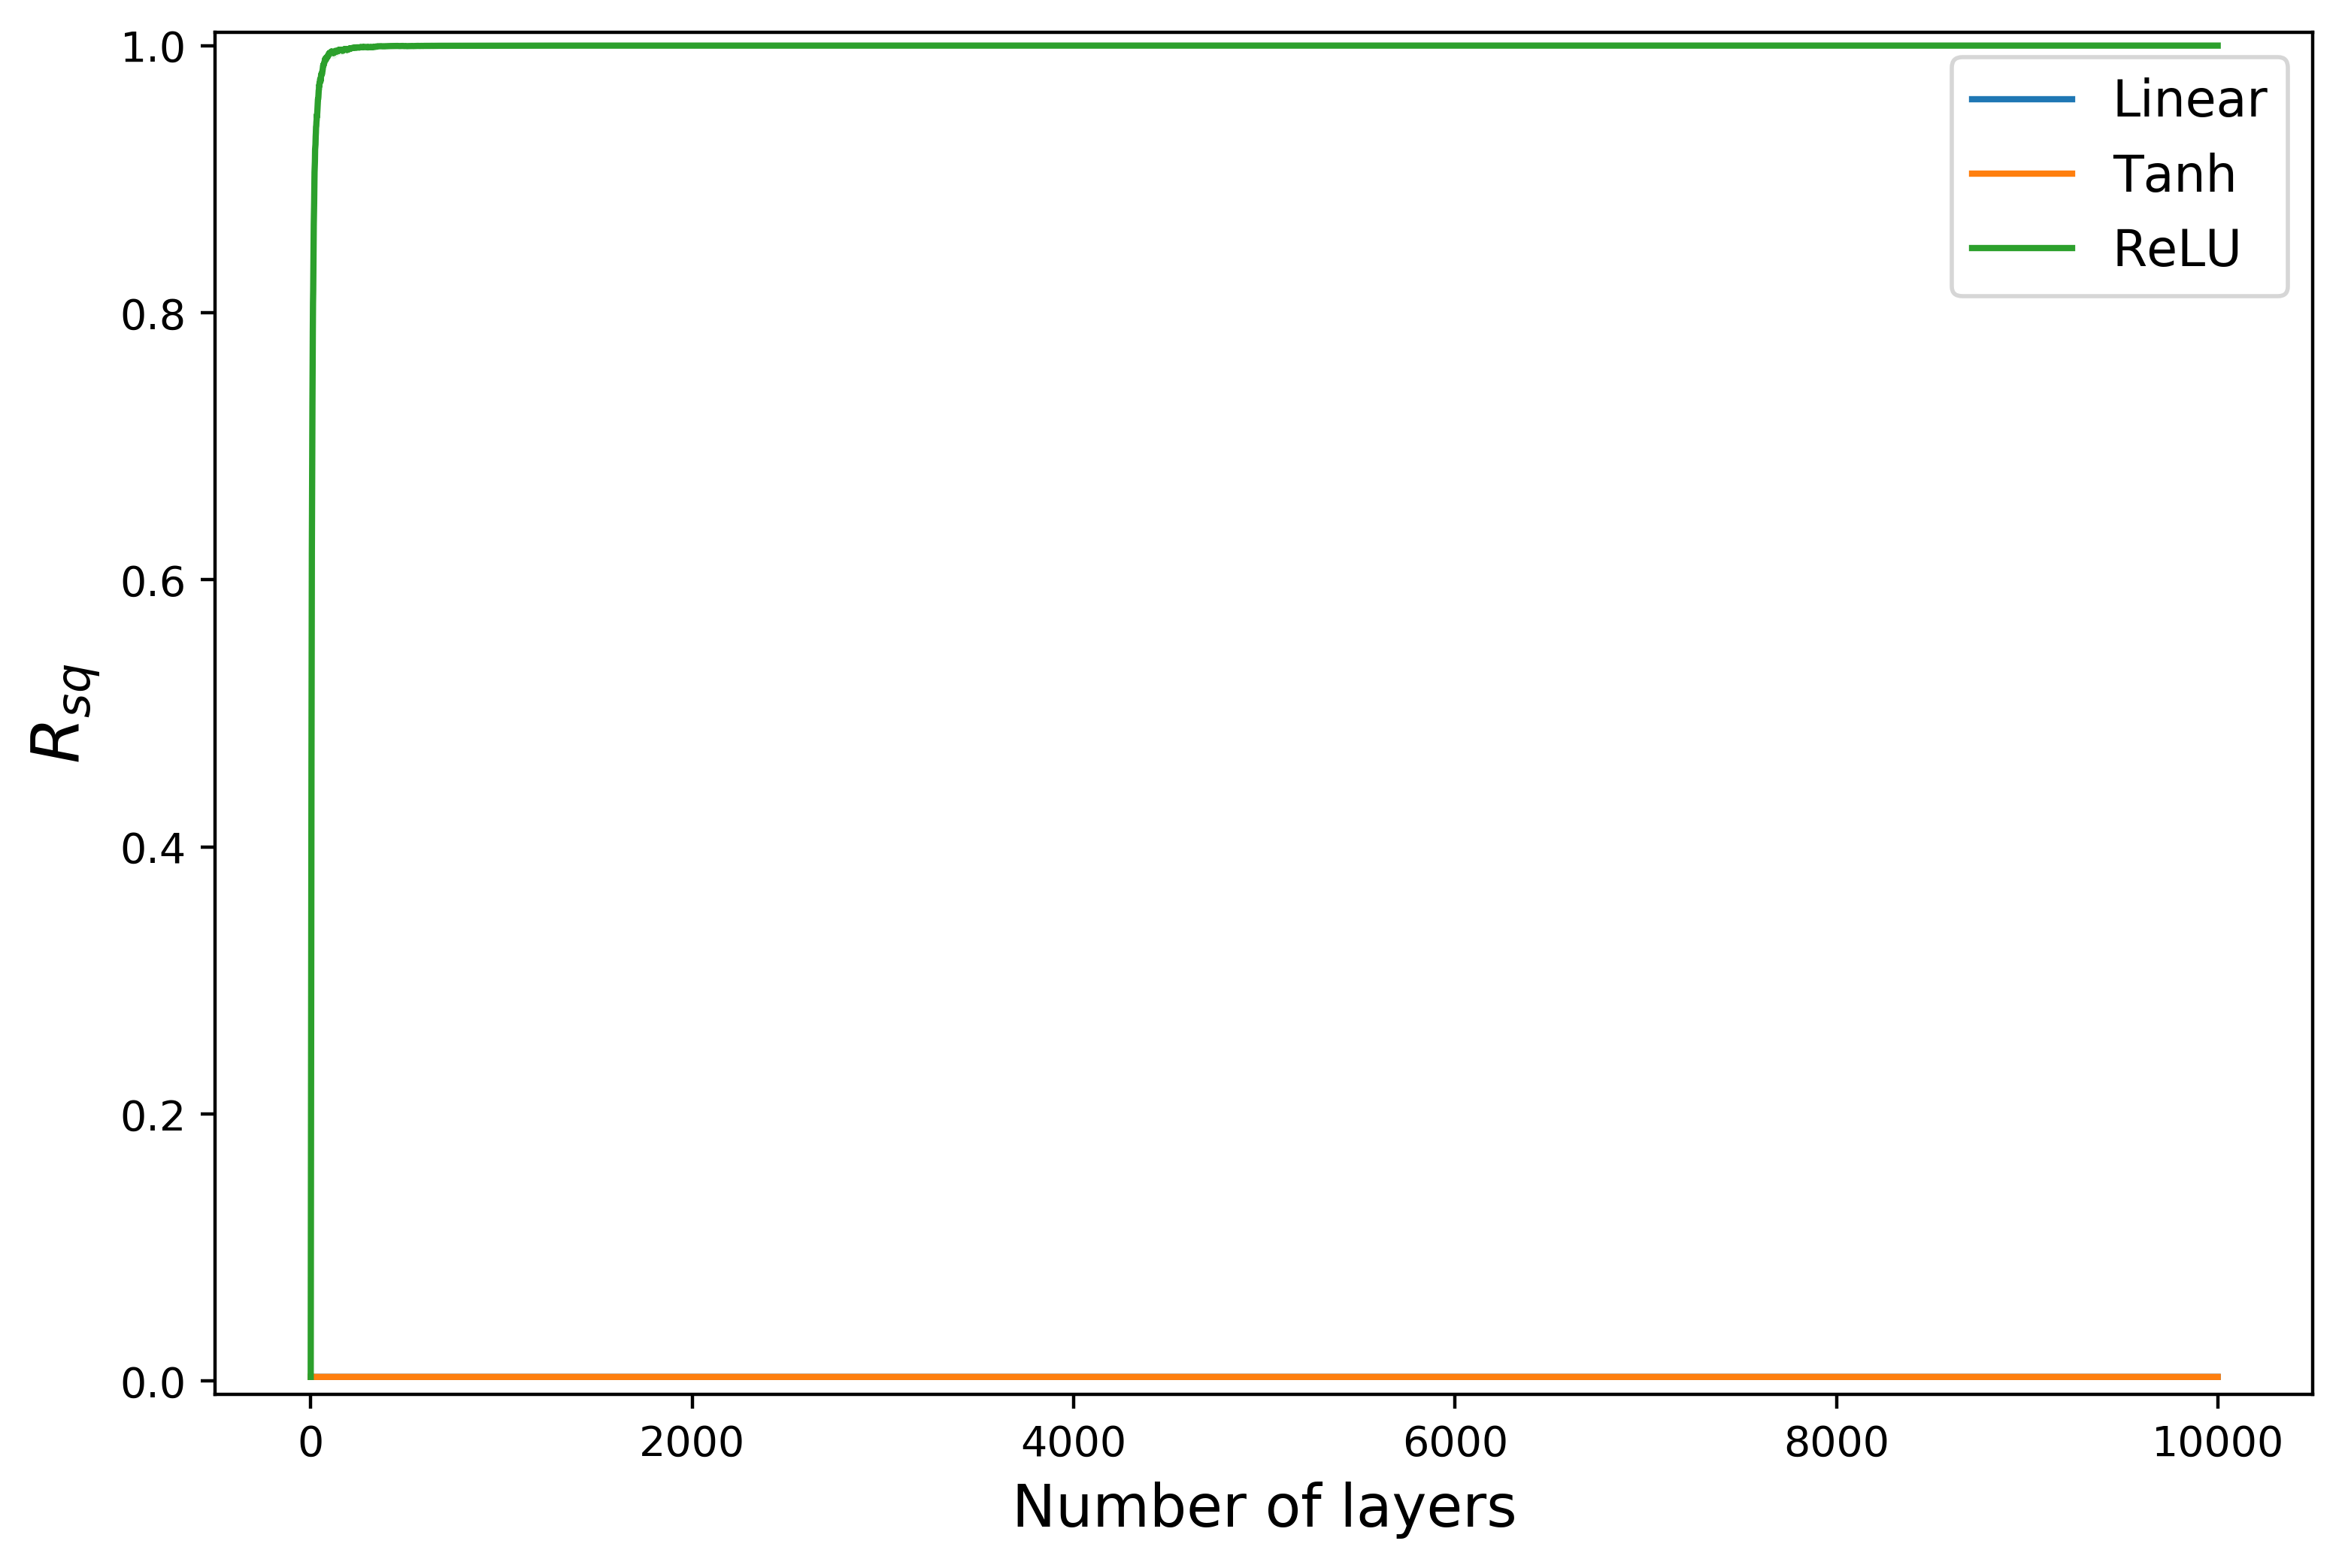
\includegraphics[width=1.0\linewidth]{10000_o_layer_rsq}
      \label{fig:repr_orthogonal_a}
    \end{subfigure}
    
    \begin{subfigure}{\myWidth}
      \centering
      \caption{Network depth $L\in[1, 500]$}
      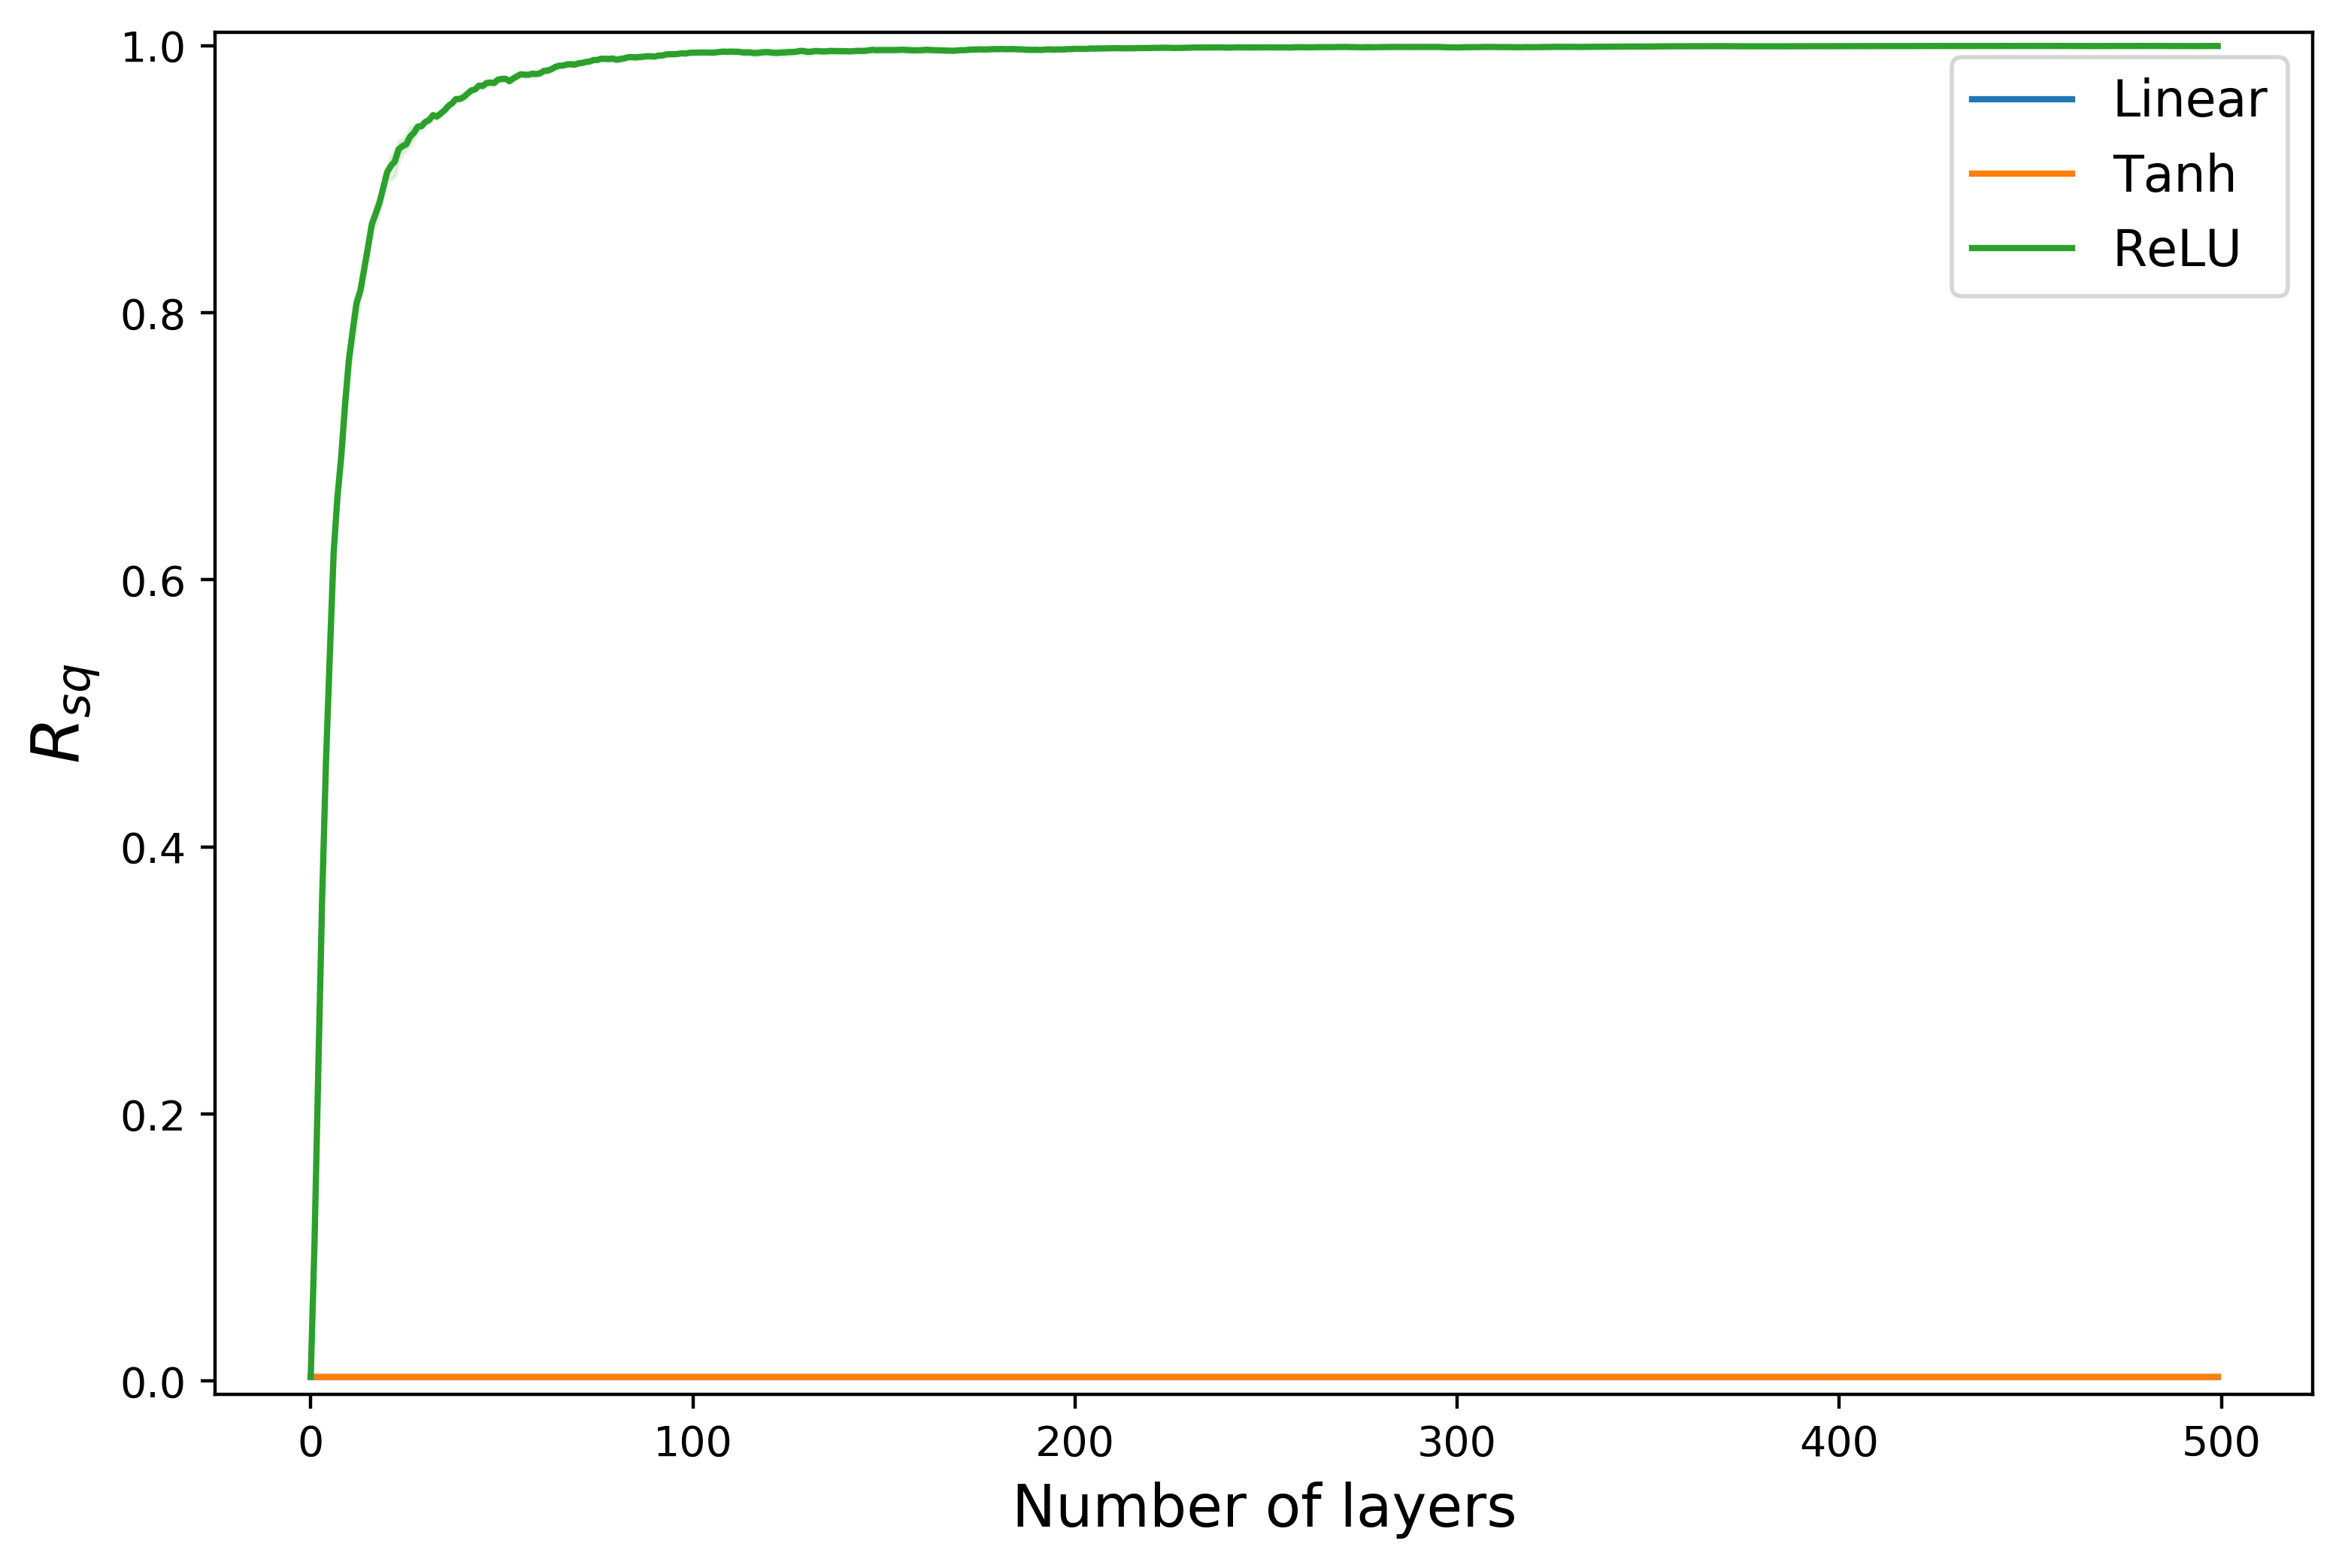
\includegraphics[width=1.0\linewidth]{500_o_layer_rsq}
      \label{fig:repr_orthogonal_b}
    \end{subfigure}%
    \caption[The initial VNI $R_{sq}$ of orthogonal initialized networks.]{
        Similar settings to Figure \ref{fig:repr_general} are used excluding the weights,
        which are initialized with scaled-Orthogonal distribution (\cite{mft:linear}).
        It is shown that for a feed-forward architecture under the orthogonal initialization
        with linear or tanh activation function, the initial VNI $R_{sq}$ remain nearly
        minimum (1/N) even when the network depth $L$ gets larger, and that the VNI of ReLU
        activation increases to 1 as the network goes deeper.
    }
    \label{fig:repr_orthogonal}
\end{figure}

\begin{figure}[h]
    \centering
    \newcommand{\myWidth}{0.48\textwidth}
    \begin{subfigure}{\myWidth}
      \centering
      \caption{Residual deep network with 1-layer skip}
      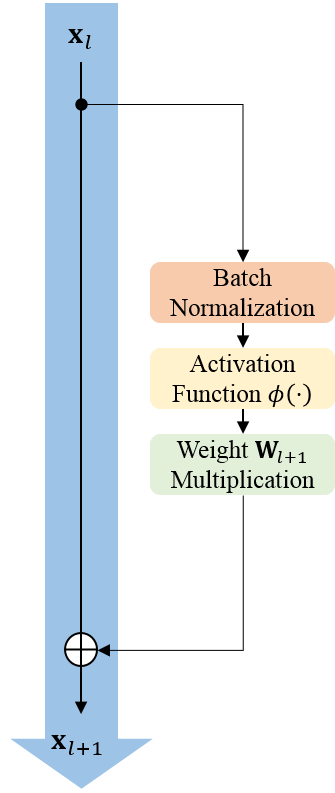
\includegraphics[width=0.48\linewidth]{architecture_res1}
      \label{fig:resnet_def1}
    \end{subfigure}
    \begin{subfigure}{\myWidth}
      \centering
      \caption{Residual deep network with 2-layer skip}
      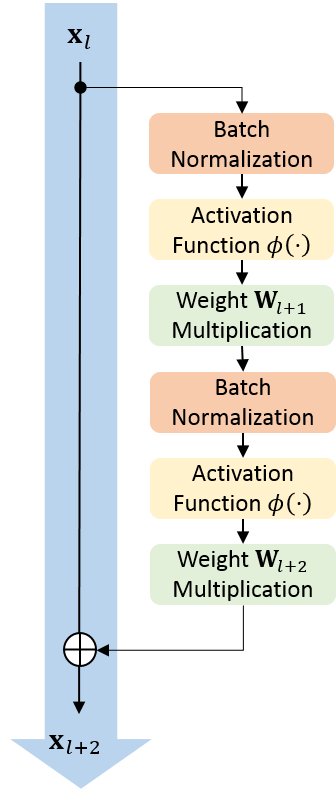
\includegraphics[width=0.48\linewidth]{architecture_res2}
      \label{fig:resnet_def2}
    \end{subfigure}%
    \caption[The architectures of residual deep networks]{
        The architectures of residual deep networks is presented in this figure.
        The network is composed of 4 operations: batch normalization (\cite{batchnorm}), activation
        function, weight multiplication and the addition with the identity mapping from the skip 
        connection.
        The left architecture has the 1-layer skip, and the right one has the 2-layer skip, which is
        the original definition in previous works(\cite{resnet2}).
    }
    \label{fig:resnet_def}
\end{figure}

\begin{figure}[h]
    \centering
    \newcommand{\myWidth}{0.9\textwidth}
    \begin{subfigure}{\myWidth}
      \centering
      \caption{1-layer shortcut defined in Figure \ref{fig:resnet_def1}}
      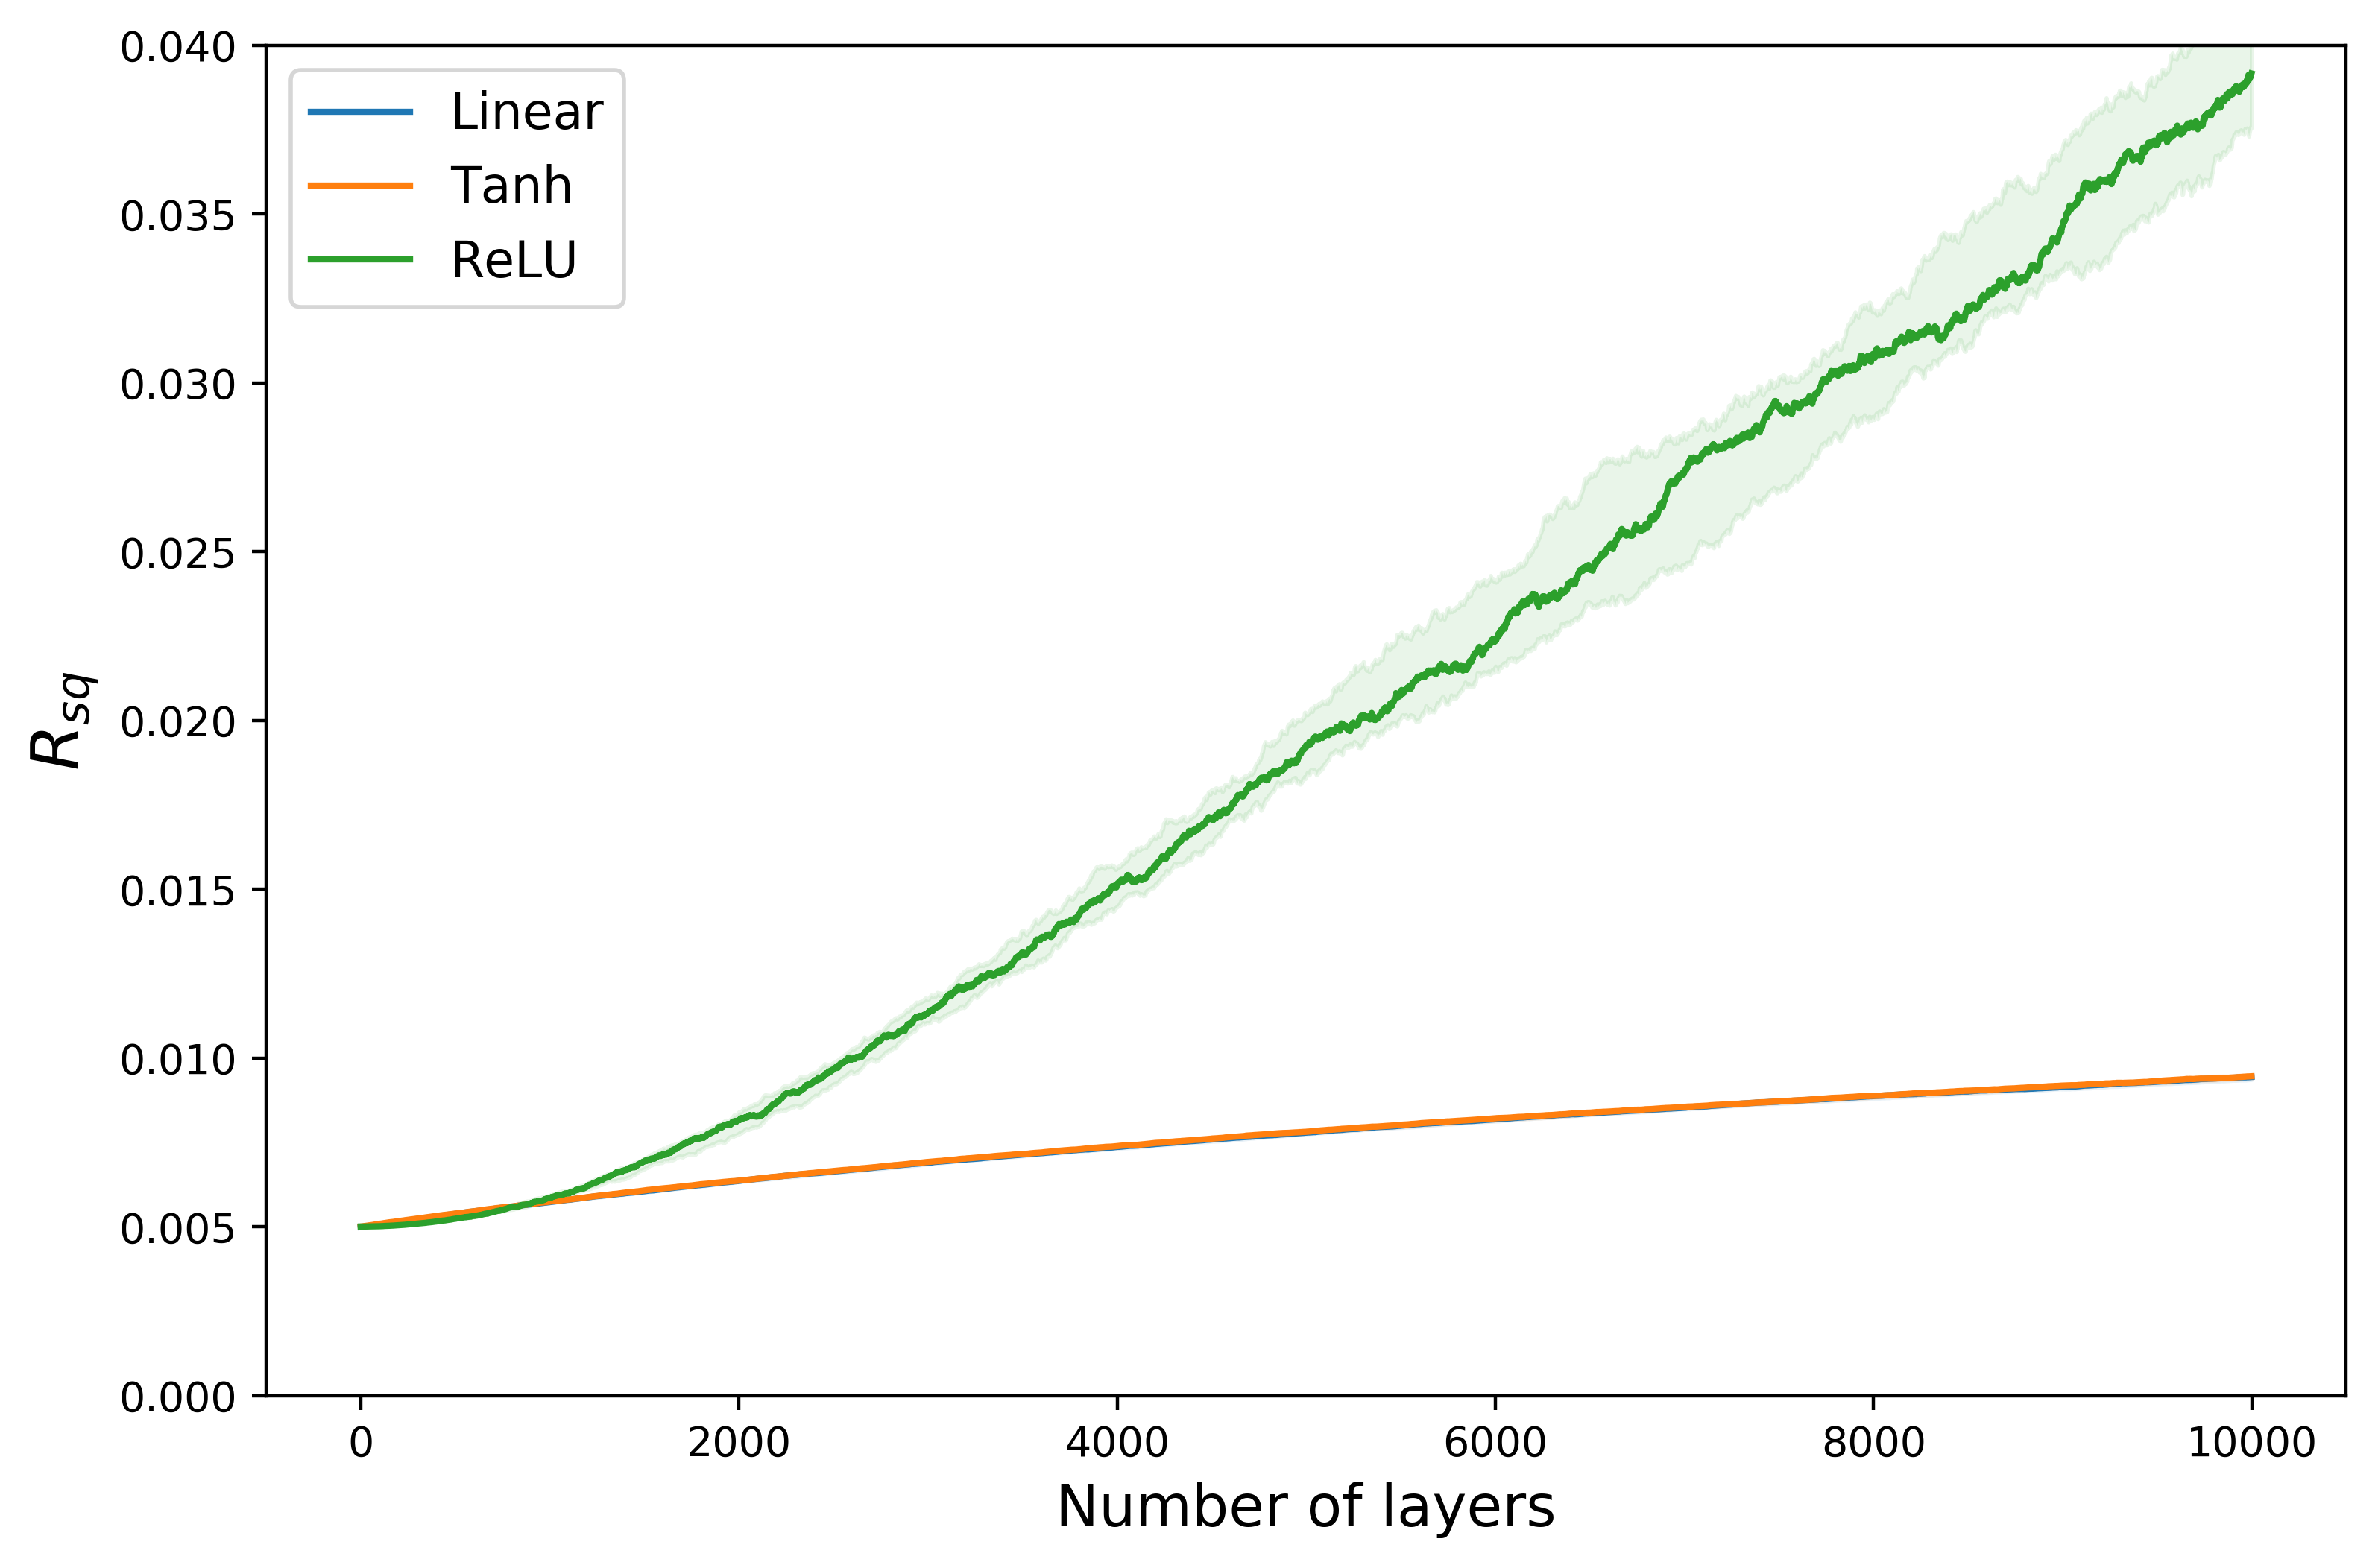
\includegraphics[width=1.0\linewidth]{10000_r1_layer_rsq}
      \label{fig:repr_residual_a}
    \end{subfigure}
    
    \begin{subfigure}{\myWidth}
      \centering
      \caption{2-layer shortcut defined in Figure \ref{fig:resnet_def2}}
      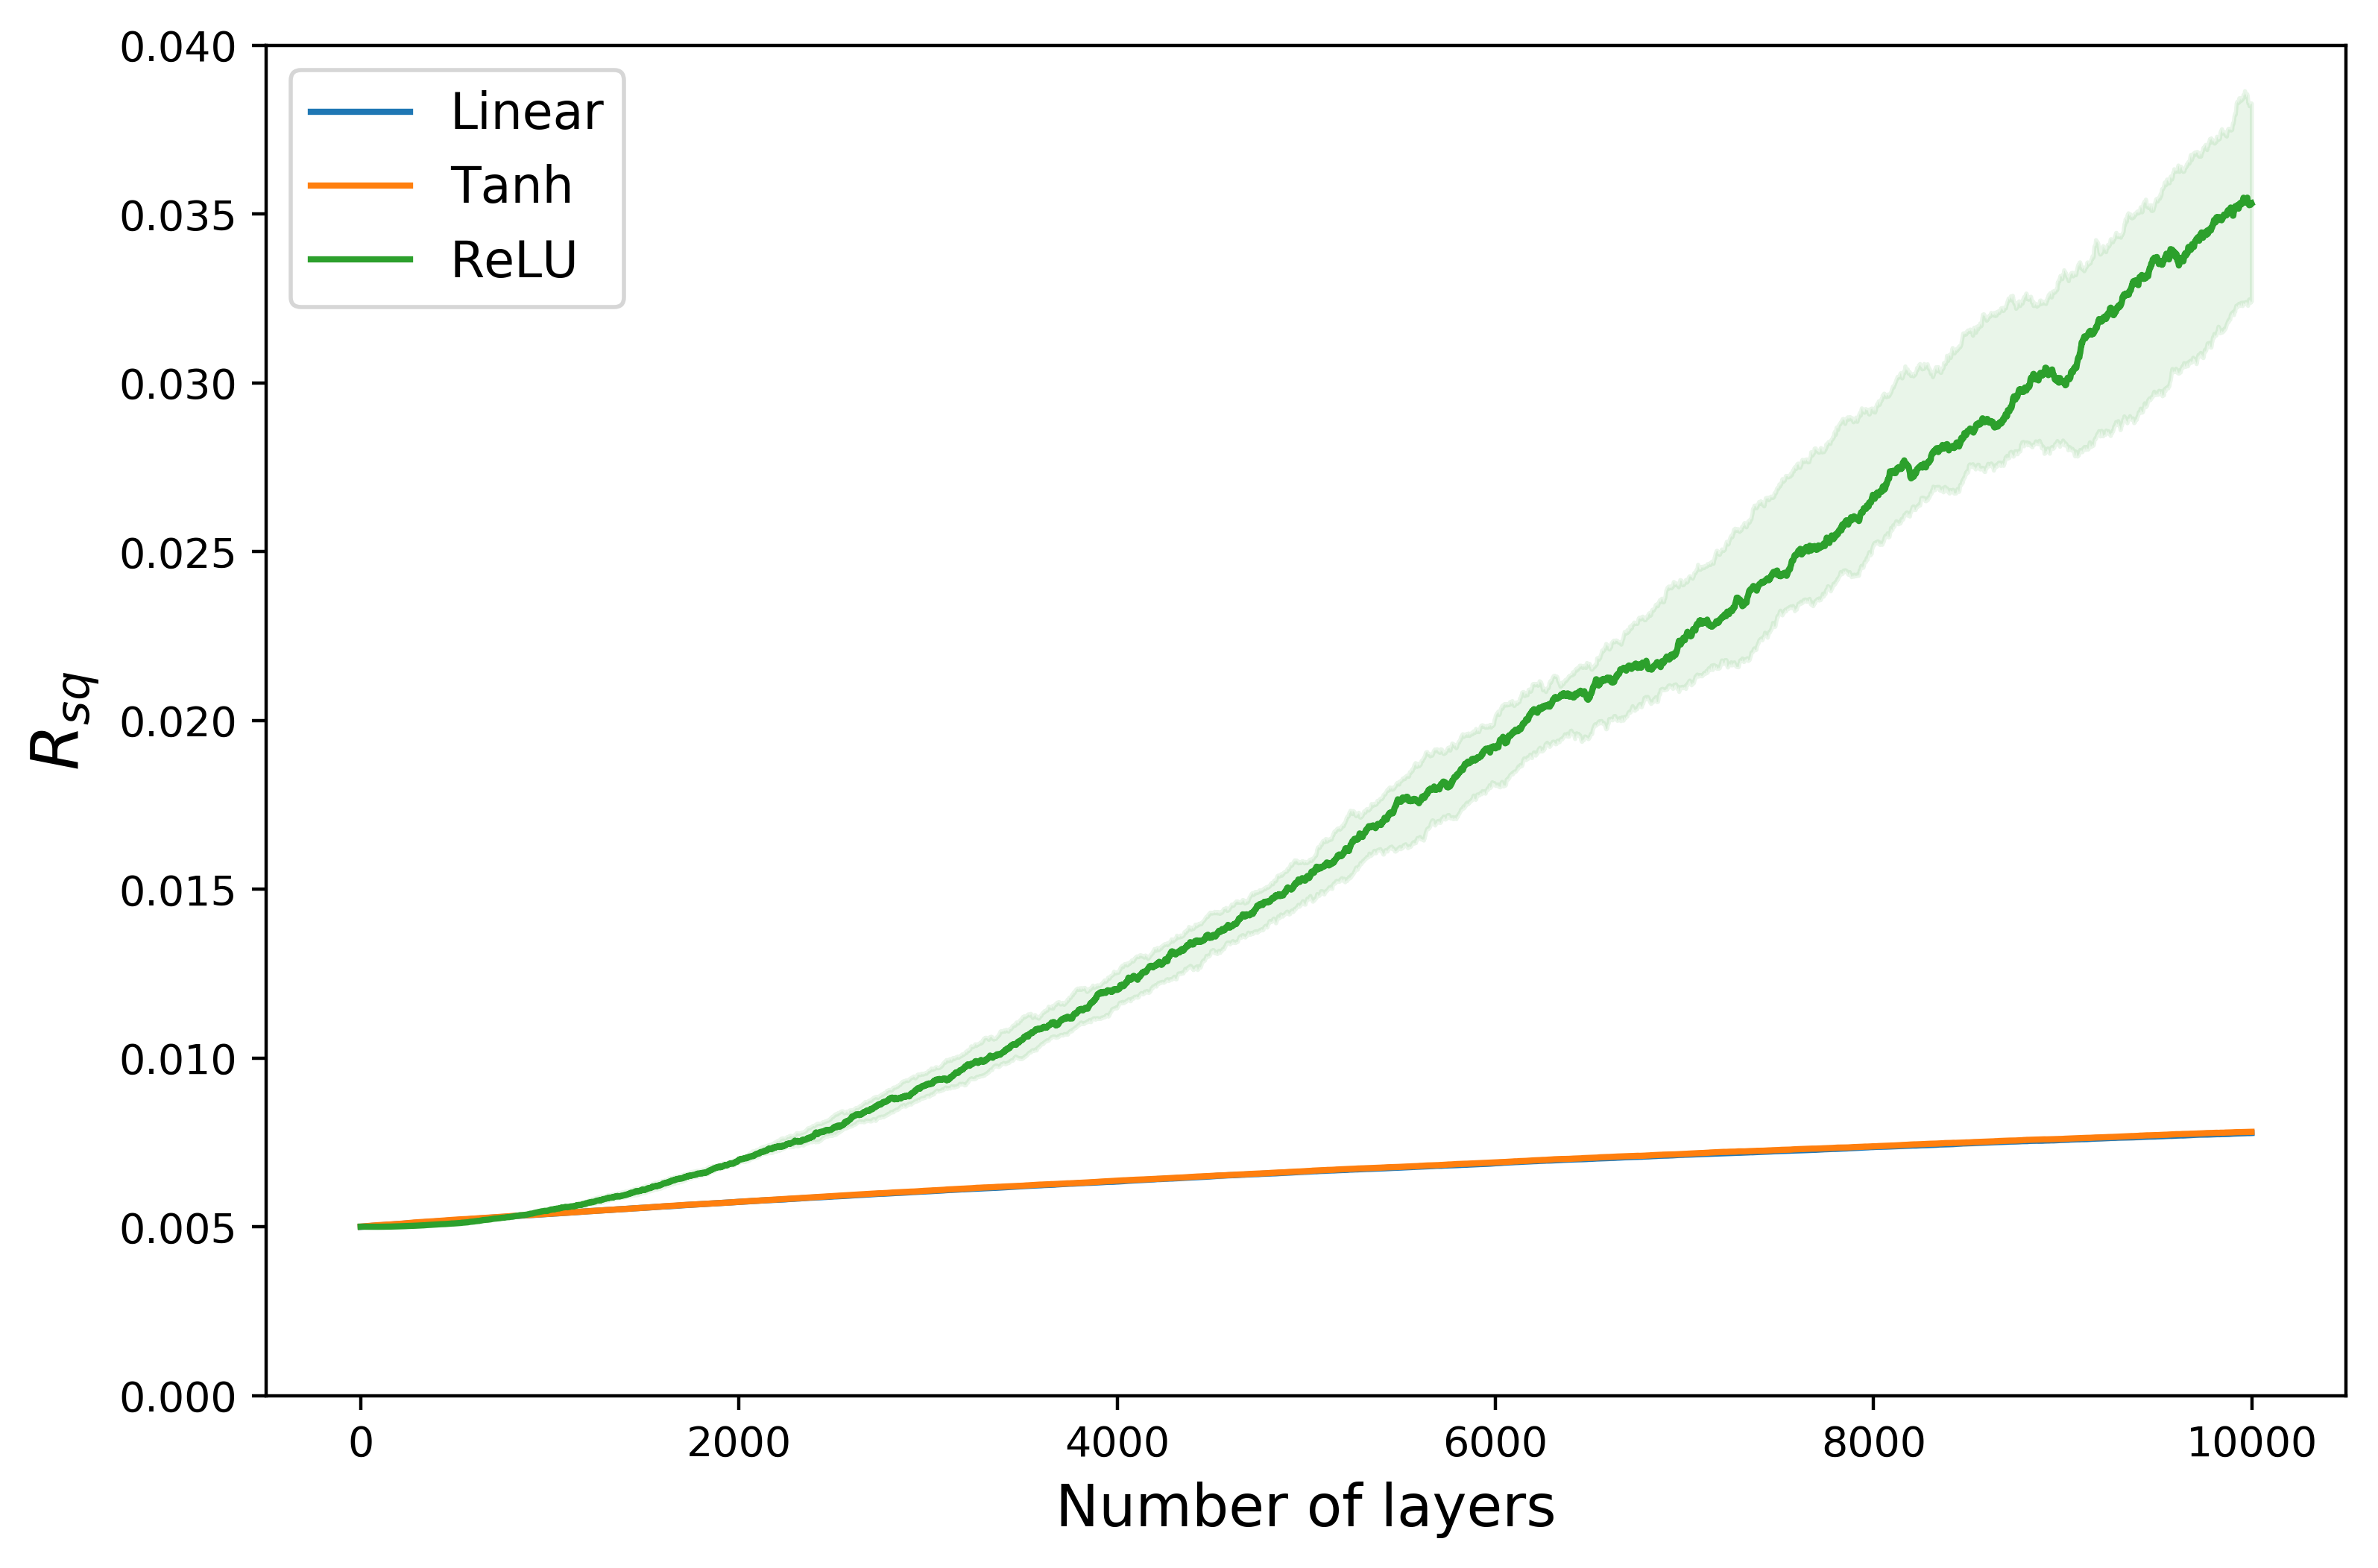
\includegraphics[width=1.0\linewidth]{10000_r2_layer_rsq}
      \label{fig:repr_residual_b}
    \end{subfigure}%
    \caption[The initial VNI $R_{sq}$ of residual networks.]{
    Similar settings to Figure \ref{fig:repr_general} are used excluding the network architectures,
    which are defined in Figure \ref{fig:resnet_def}.
    It is shown that for a residual-like architecture, the VNI $R_{sq}$ grows slowly as the network
    depth $L$ gets larger.
    Note that for the 2-layer shortcut architecture, we only perform the simulation with even numbers
    of hidden layers.}
    \label{fig:repr_residual}
\end{figure}


\begin{figure}[h]
    \centering
    \newcommand{\myWidth}{0.9\textwidth}
    \begin{subfigure}{\myWidth}
      \centering
      \caption{Tanh activatoin function}
      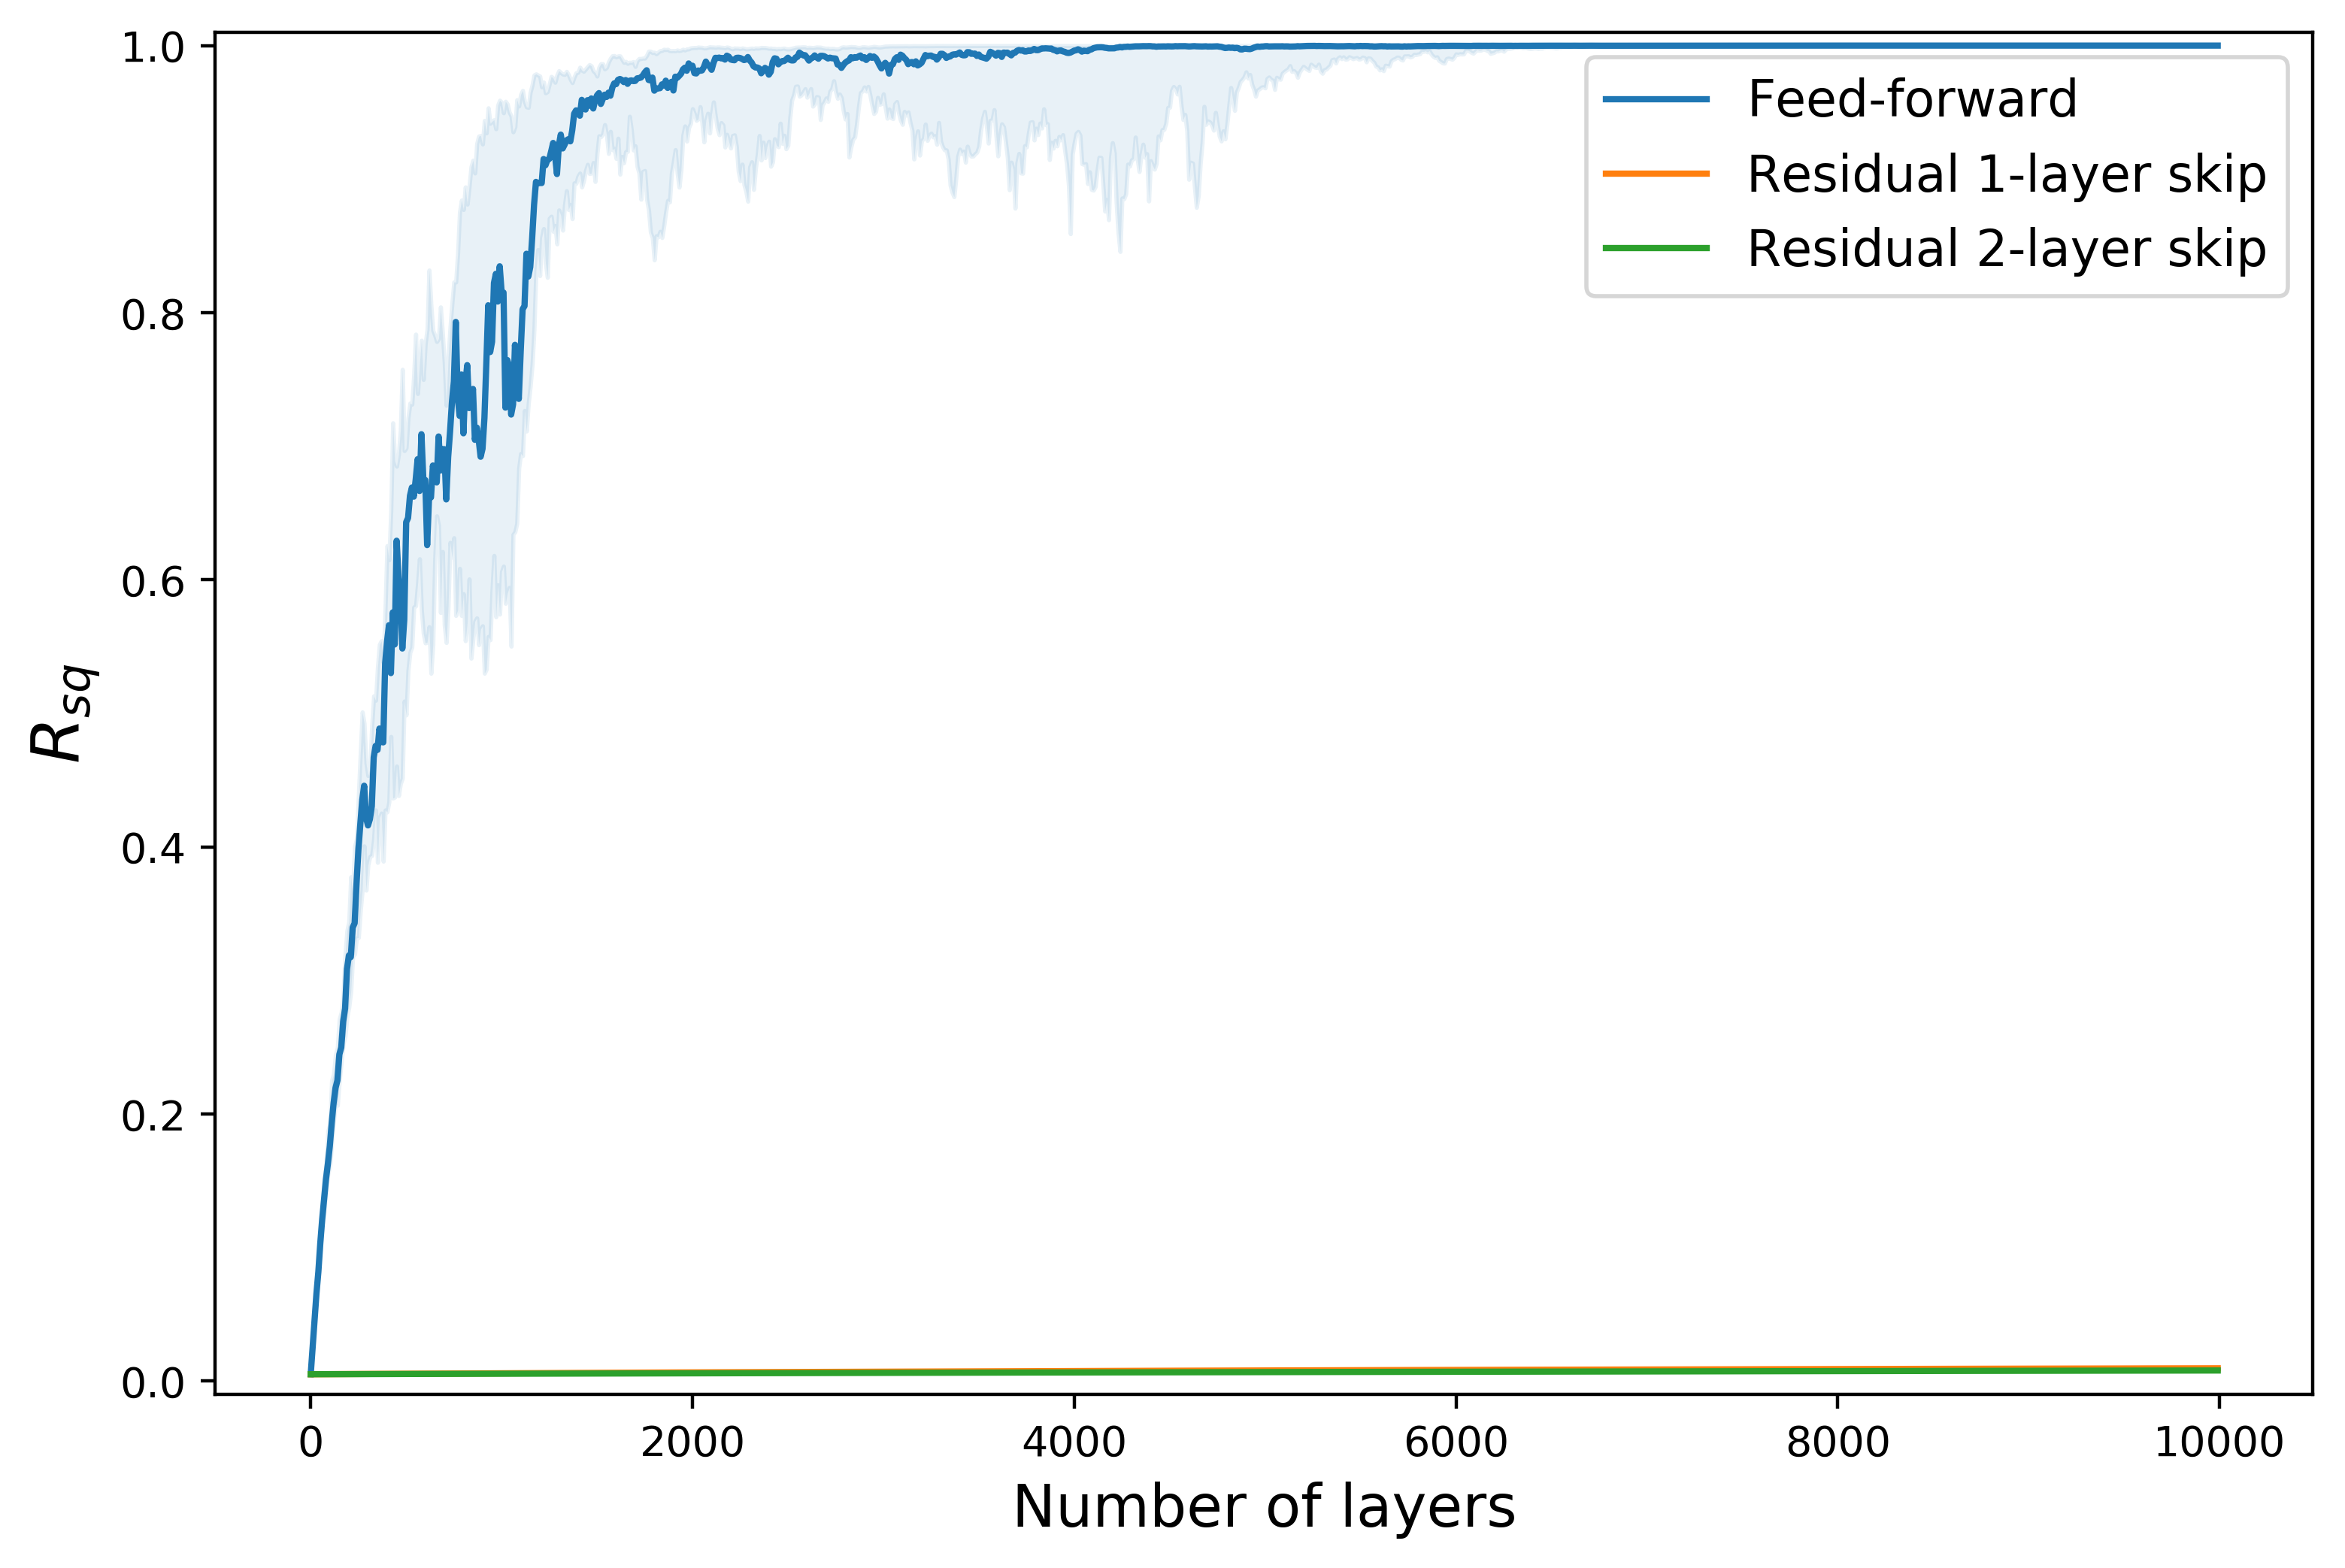
\includegraphics[width=1.0\linewidth]{10000_tanh_layer_rsq}
      \label{fig:repr_architecture_a}
    \end{subfigure}
    
    \begin{subfigure}{\myWidth}
      \centering
      \caption{ReLU activation function}
      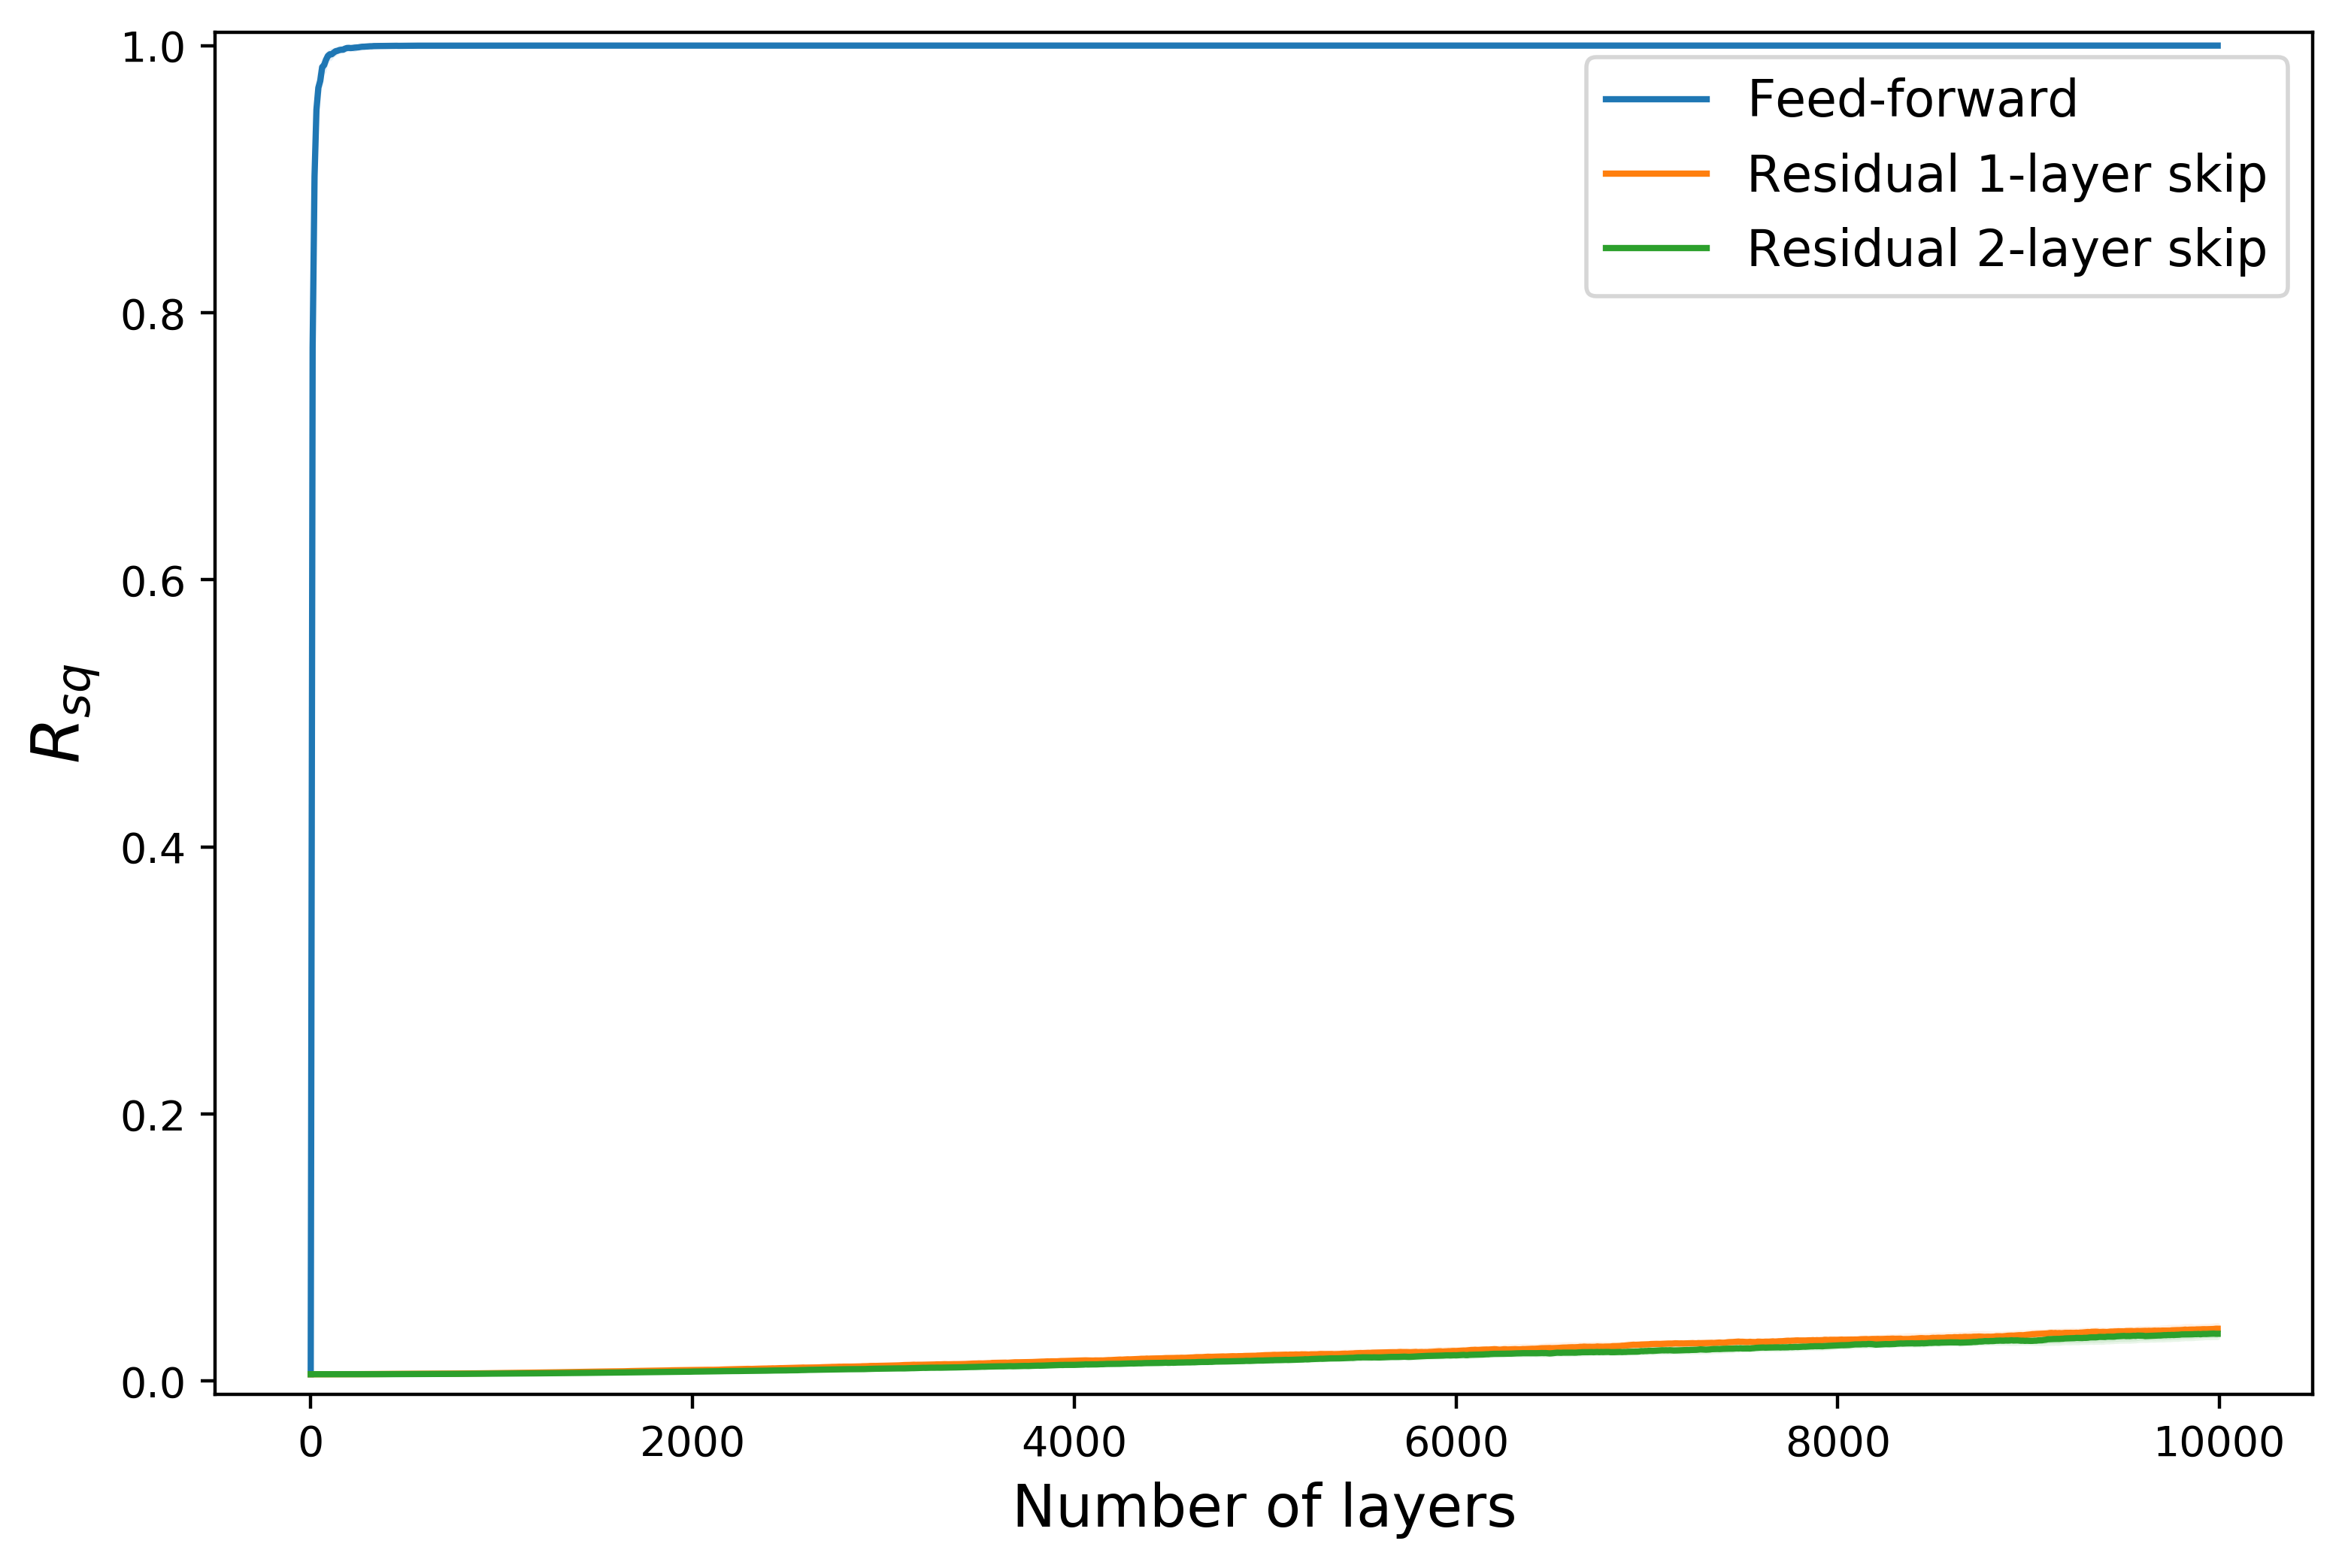
\includegraphics[width=1.0\linewidth]{10000_relu_layer_rsq}
      \label{fig:repr_architecture_b}
    \end{subfigure}%
    \caption[The initial VNI $R_{sq}$ of different network architectures.]{
    To compare the VNI $R_{sq}$ of different network architectures, we plot the curves of Figure
    \ref{repr_general} and \ref{repr_residual} in the same graph.
    The weight initialization methods are set to the same (Gaussian distribution).
    We can see that for both tanh and ReLU cases, the residual architecture has much smaller VNI
    $R_{sq}$ when the network depth $L$ increases.
    It implies that the residual skip connections can keep more representation power when a very deep
    network is considered.
    }
    \label{fig:repr_architecture}
\end{figure}


\begin{figure}[h]
    \newcommand{\myWidth}{0.9\textwidth}
    \centering
    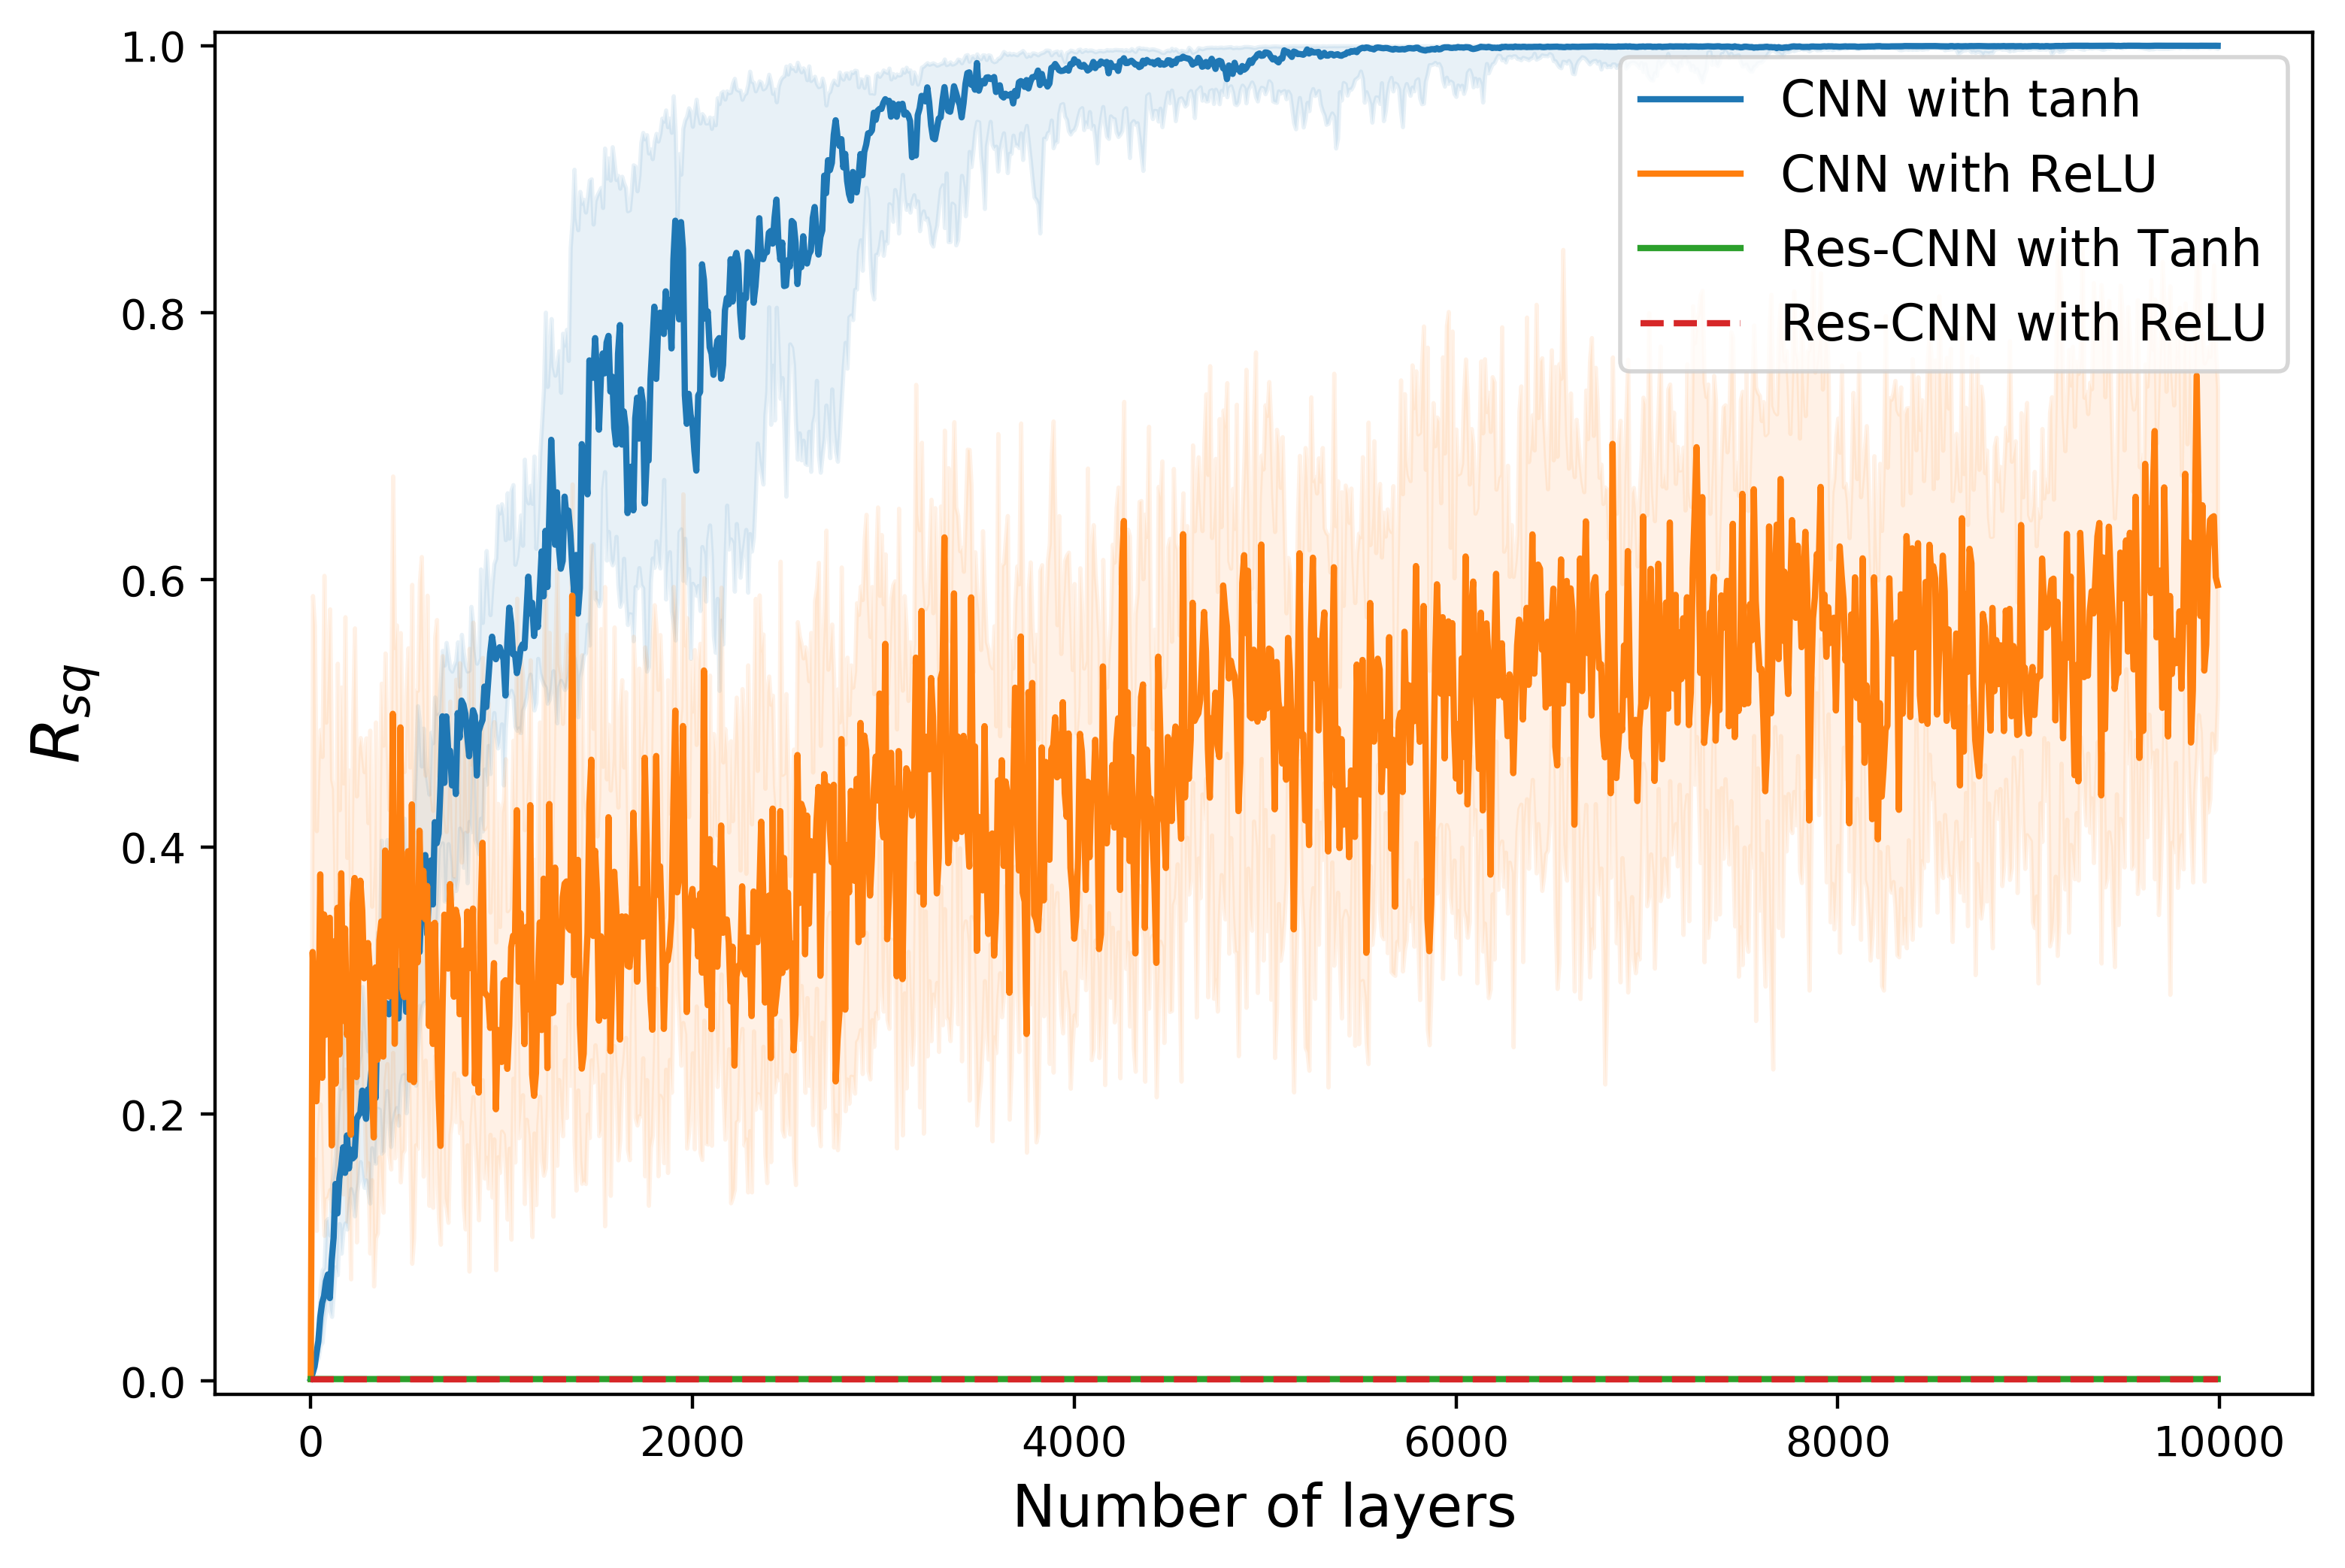
\includegraphics[width=\myWidth]{10000_cnn_layer_rsq}
    \caption[The initial VNI $R_{sq}$ of convolutional neural networks.]{
    To compare the VNI $R_{sq}$ of different network architectures of convolutional neural networks,
    we plot the results of architectures with and without residual connection.
    The weight initialization methods are set to the same (Gaussian distribution).
    Similar to Figure \ref{fig:repr_architecture}, we can see that for both tanh and ReLU cases,
    the residual architecture has much smaller VNI $R_{sq}$ when the network depth $L$ increases.
    Also, compared with the feed-forward deep neural network in Figure \ref{fig:repr_architecture},
    the VNI $R_{sq}$ increases slower with respect to the network depth $L$.
    It implies that the residual skip connections and the convolution operation can keep more
    representation power when a very deep network is considered.
    }
    \label{fig:repr_cnn}
\end{figure}


\begin{table}[h]
    \centering
    \begin{tabular}{|l|l|r|r|}
    \hline
        Activation & $\phi(x)$ & $\mu_k$ & Norm-preserving $\sigma_w^2$\\\hline
        Linear & $x$ & $1$ & $1$\\\hline
        ReLU & $[x]_{+}$ & $1/2$ & $2$\\\hline
        Hard Tanh & $[x+1]_{+}-[x-1]_{+}-1$ & $erf\Big(\frac{1}{\sqrt{2}\sigma}\Big)$
        & $erf\Big(\frac{1}{\sqrt{2}\sigma}\Big)^{-1}$\\\hline
    \end{tabular}
    \caption[The $\mu_k$ of different activation functions.]
    {The $\mu_k$, the $k$-th moments of series expansion of the moment generating function
    associated with activation functions, is provided in this table.
    The derivation is given by \cite{mft:spectral}.
    The rightmost column are the norm-preserving $(\sigma_w^2)$, which will be further
    discussed in \ref{comp:init}.
    Note that the $\sigma^2$ is the variance of the hidden nodes.
    It shows that the maximal depth of ReLU activation is much less than linear and tanh
    activations, and that the orthogonal weights and the residual architecture can improve
    the maximal depth of networks.}
    \label{table:mu}
\end{table}


\begin{table}[h]
    \centering
    \begin{tabular}{|l|r|}
    \hline
        Random Matrix $W$ & $s_1$\\\hline
        Gaussian & $-1$\\\hline
        Orthogonal & $0$\\\hline
    \end{tabular}
    \caption[The $s_1$ of different weight distribution.]
    {The $s_1$ of different activation functions.
    The derivation is given by \cite{mft:spectral}.
    Note that the $s_1$ is invariant to the matrix scale. That is, the results are also
    suitable for the scaled-Gaussian and the scaled-orthogonal initializations.}
    \label{table:s}
\end{table}

\begin{table}[h]
    \centering
    \begin{tabular}{|c|c|c|r|}
    \hline
        Architecture&Weight initialization.&Activation&Maximal depth\\\hline
        \multirow{6}{*}{Feed-forward network} & \multirow{3}{*}{Scaled Gaussian} & tanh & 4243\\\cline{3-4}
         &  & linear & 2606\\\cline{3-4}
         &  & relu   & 262 \\\cline{2-4}
         & \multirow{3}{*}{Orthogonal} & tanh   & $>10000$\\\cline{3-4}
         &  & linear & $>10000$\\\cline{3-4}
         &  & relu   & 325\\\hline
         \multirow{3}{*}{Residual network} & \multirow{3}{*}{Scaled Gaussian} & tanh   & $>10000$\\\cline{3-4}
         &  & linear & $>10000$\\\cline{3-4}
         &  & relu   & $>10000$\\\hline
    \end{tabular}
    \caption[The maximum depth for different architectures and initializations]
    {The maximum depth for representation power. The maximum depth
    is defined as the maximal $L$ such that in less than half of 20
    runs(i.e. 10 runs), the approximated number of effective nodes achieve greater than 1.}
    \label{dead_table}
\end{table}

